\documentclass[12pt,a4paper]{article} %12 кегль, формат бумаги А4, тип статья

\usepackage[T2A]{fontenc} %поддержка кириллицы
\usepackage[utf8]{inputenc} %кодировка символов юникод
\usepackage[english,russian]{babel} %список рабочих языков
\usepackage{cmap} %для поиска в pdf
\usepackage[left=2cm,right=2cm,top=2cm,bottom=2cm]{geometry} %размеры отступов от краев страницы
\usepackage{graphicx} %возможность работать с графикой
\usepackage{enumitem} %для работы со списками
\usepackage{float} %для точного размещения таблиц и графики
\usepackage{caption} %для создания подписей таблиц и графики
\usepackage{amsmath,amssymb,amsthm,amsfonts} %штуки для математики
\usepackage{extarrows} %чтобы подписи над и под нестандартными стрелками писать короче в коде
\usepackage{makeidx} %собирает ключевые слова для предметного указателя
\usepackage[hidelinks]{hyperref} %убирает выделение ссылок; добавляет гиперссылки в оглавление, перекрестные ссылки и URL
\usepackage{setspace} %устанавливает отступы
\linespread{1.5} %длина межстрочного интервала
\vspace{125mm} %длина абзацного отступа
\usepackage{titlesec}
\titleformat{\section}{\normalfont\Large\bfseries\centering}{}{0pt}{} % эти две строчки убирают циферки перед названиями разделов в основном тексте и выравнивают названия секций по центру
\titleformat{\part}{\normalfont\LARGE\bfseries\centering}{}{0pt}{}
\usepackage{paratype} %чтобы точно был поиск и шрифт хороший

\author{Автор конспекта: Краснов Б. А.}
\title{Давыдов Ю.А.: Теория мартингалов}
\date{весна 2026}

\newtheorem{theorem}{Теорема}
\newtheorem{lemma}{Лемма}
\newtheorem{definition}{Определение}
\newtheorem{proposition}{Предложение}
\newtheorem{consequence}{Следствие}
\newcommand{\R}{\mathbb{R}}
\newcommand{\Co}{\mathbb{C}}
\newcommand{\E}{\mathbb{E}}
\newcommand{\D}{\mathbb{D}}
\newcommand{\PR}{\mathbb{P}}
\newcommand{\charf}[2][t]{\varphi_{#2}(#1)}
\newcommand{\F}{\mathcal{F}}
\newcommand{\M}{\mathfrak{M}}

\begin{document}
	\maketitle
	\begin{figure}[H]
		\centering
		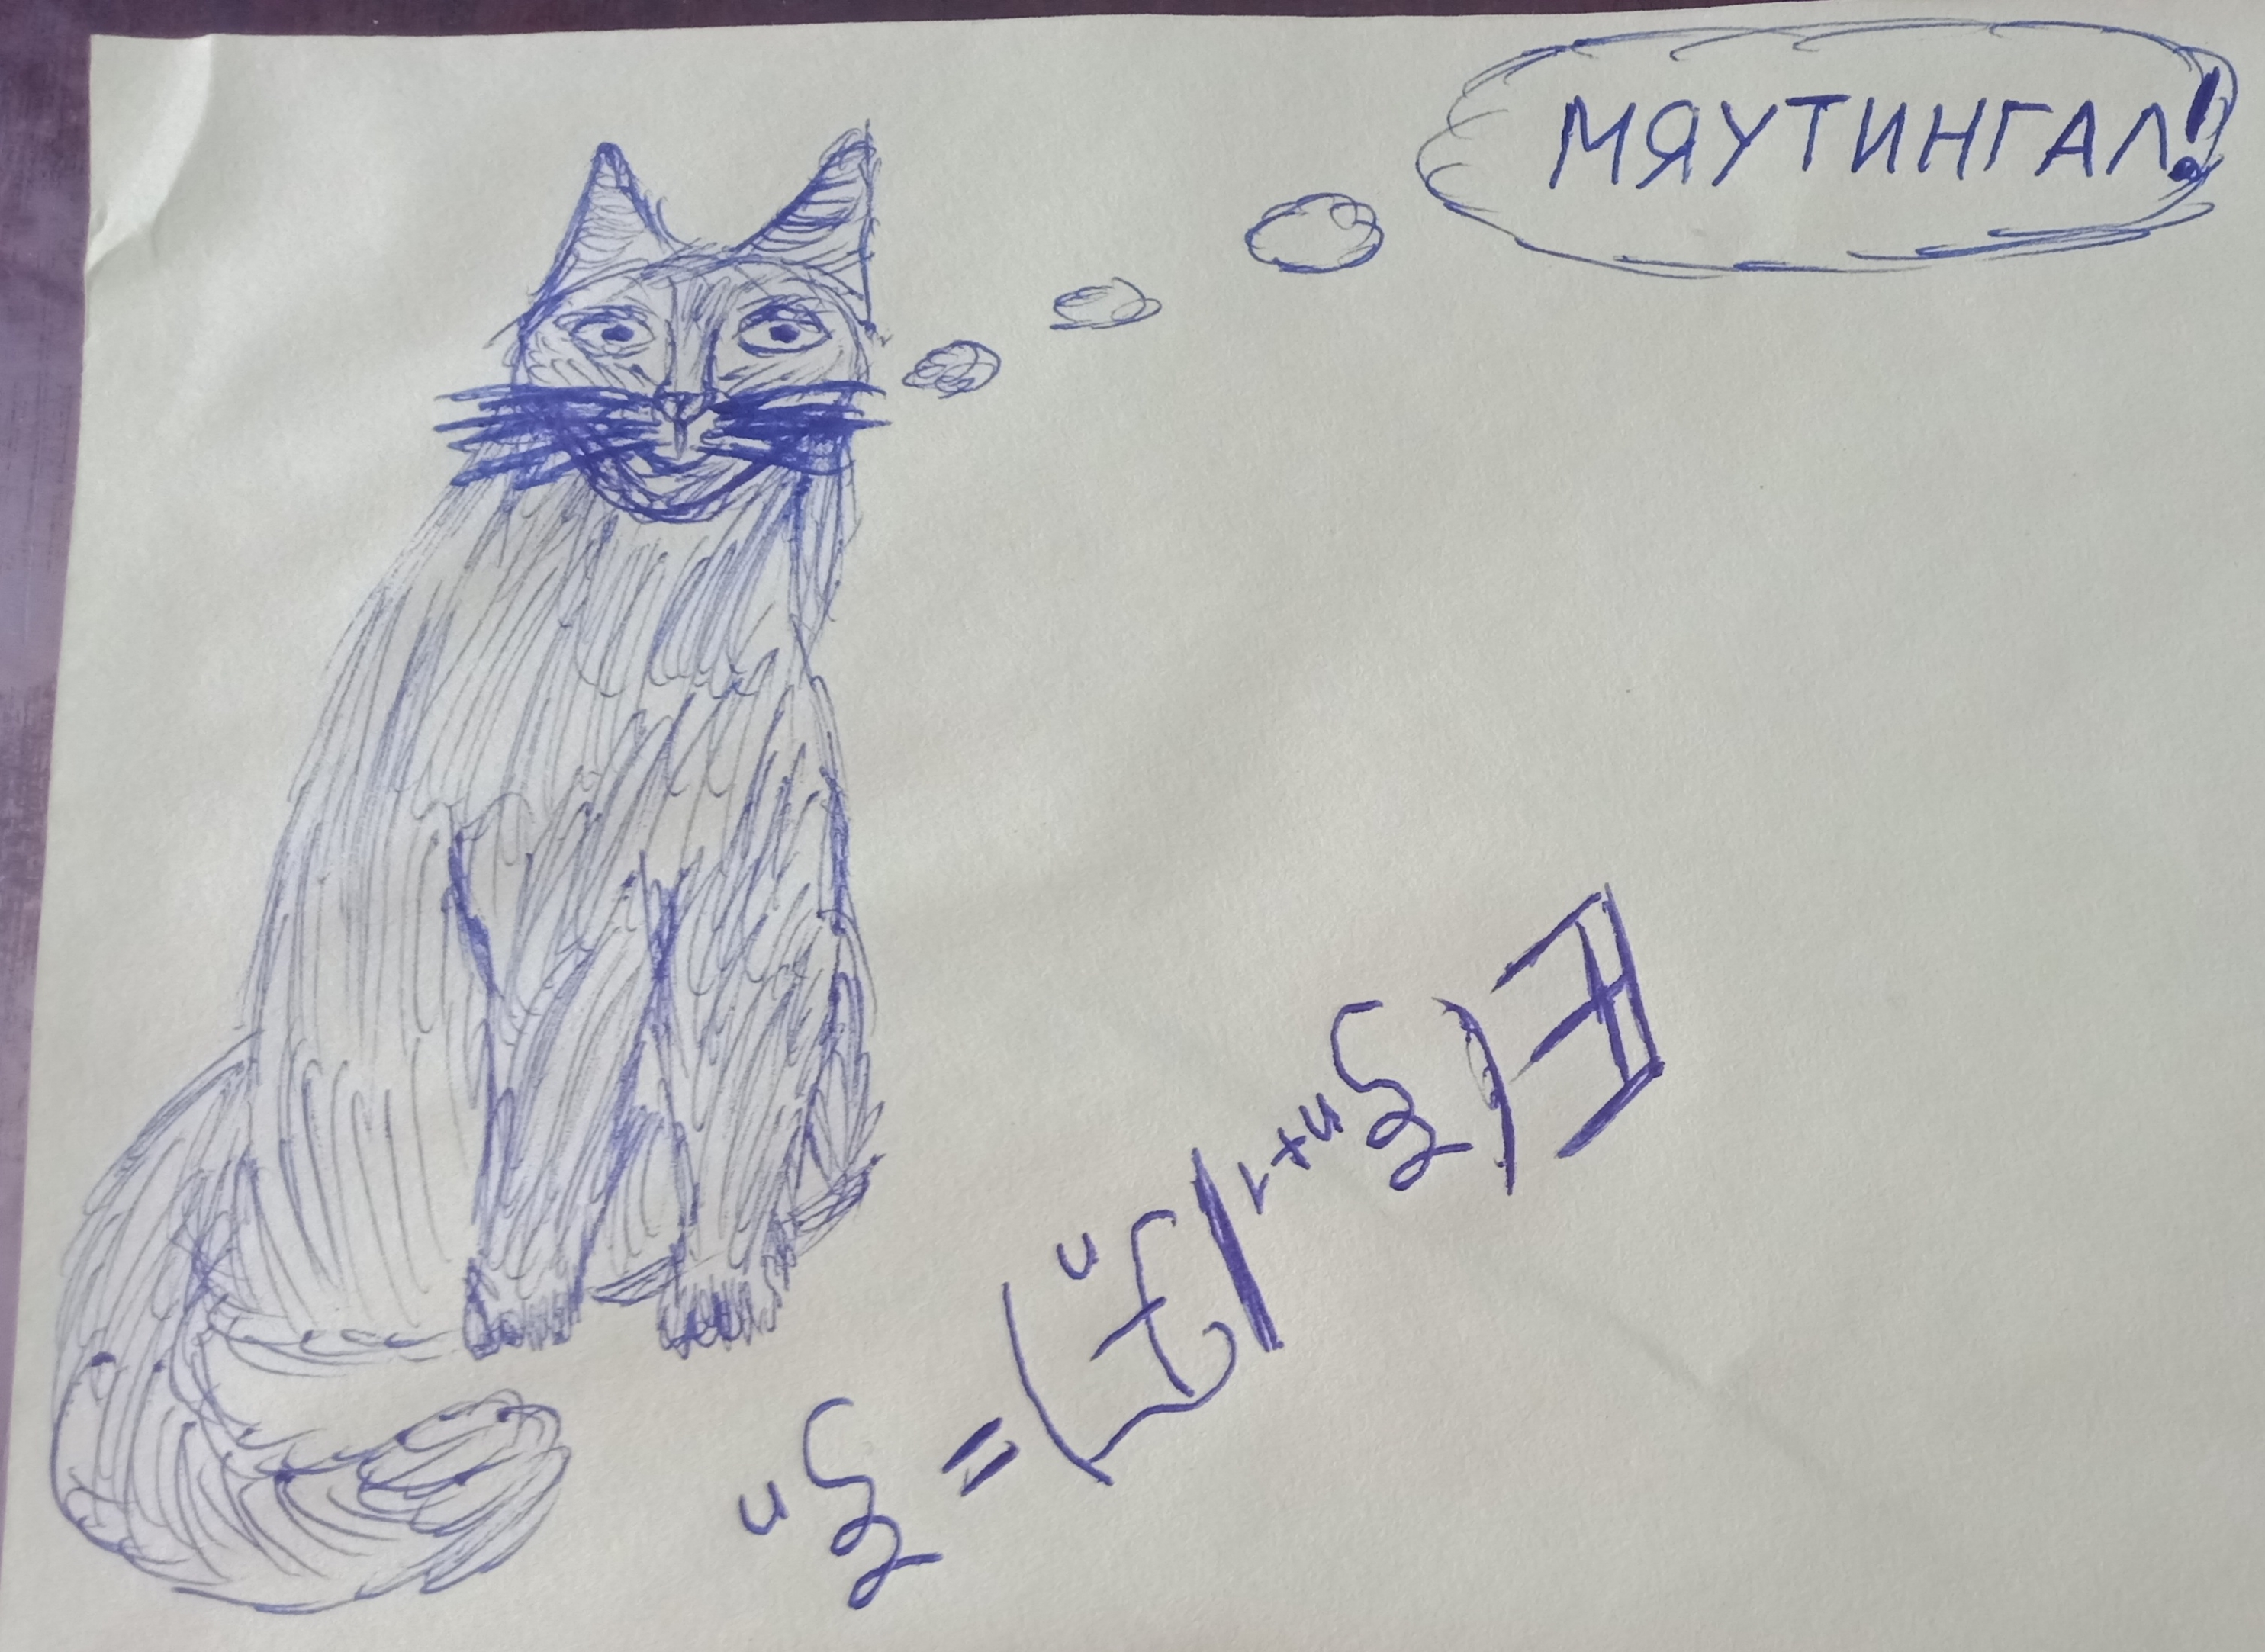
\includegraphics[scale=0.15]{котик_мартингал.jpg}
		\caption*{\LARGE Котик для Лизы!}
	\end{figure}
	\tableofcontents
	\clearpage
	\part{Мартингалы с дискретным временем}
	\section{Напоминание про УМО}
	Пусть $(\Omega,\F,\PR)$ - вероятностное пространство, $\xi$ - случайная величина, $\mathfrak{M}\subset\F$ - под-$\sigma$-алгебра.
	\begin{definition}
		Случайная величина $\E(\xi\vert\mathfrak{M})$ называется условным математическим ожиданием $\xi:\exists\E\xi$, если:
		\begin{enumerate}
			\item она $\mathfrak{M}$-измерима;
			\item $\forall\,A\in\mathfrak{M}\quad\displaystyle\int\limits_A\E(\xi\vert\mathfrak{M})d\PR=\int\limits_A\xi d\PR$.
		\end{enumerate}
	\end{definition}
	Теперь докажем существование условного мат. ожидания не через т. Радона-Никодима.
	\begin{proof}
		Сначала разберем приятный случай в Гильбертовом пространстве\\ $(\xi\in L^2)$. Положим в качестве условного мат. ожидания величину $\E(\xi\mid\M):=Pr_H\xi,$\\$H:=L^2(\Omega,\M,\PR)$ и проверим что она подходит. Измеримость очевидна, разберемся с интегралом.
		$$A\in\M:\,\,\,\int\limits_A\E(\xi\mid\M)d\PR=\E(I_A\E(\xi\mid\M))=[I_A,Pr_H\xi]=[Pr_HI_A,\xi]=[I_A,\xi]=\int\limits_A\xi d\PR$$
		Теперь пусть $\xi\notin L^2,\,\E\xi<\infty$. Давайте считать $\xi$ постоянного знака, а в общем случае надо разбивать случайную величину на положительную и отрицательную часть и делать для них одинаковые вещи, а потом сложить. Тогда из существования мат. ожидания существует последовательность $\{\xi_n\}_{n=1}^{+\infty}$ возрастающих простых случайных величин, которые стремятся к $\xi$ (п.н), а также имеющие все моменты, то есть по предыдущему имеют $\E(\xi_n\mid\M)$, которые также возрастают. Тогда последовательность условных мат. ожиданий сходится в $L^1$ к некоторой величине $\eta$ по теореме Леви, которая и будет условным мат. ожиданием $\xi$.
	\end{proof}
	Бонус от меня (а то какой-то короткий раздел и не полный по смыслу): не самые очевидные и важные свойства УМО (некоторые используем дальше):
	\begin{enumerate}
		\item $\E\E(\xi\mid\M)=\E\xi$;
		\item $\F_1\subset\F_2\Rightarrow\E(\E(\xi\mid\F_2)\mid\F_1)=\E(\xi\mid\F_1)$;
		\item $\F_2\subset\F_1\Rightarrow\E(\E(\xi\mid\F_2)\mid\F_1)=\E(\xi\mid\F_2)$;
		\item $\xi:\exists\E\xi,\,\forall\, A\in\M\,\,\xi,I_A$ - независимы, то $\E(\xi\mid\M)=\E\xi$;
		\item $\eta - \M$ - измеримая, $\E|\xi|<+\infty,\,\E|\xi\eta|<+\infty$, тогда $\E(\xi\eta\mid\M)=\eta\E(\xi\mid\M)$;
		\item $\xi - \M$ - измерима, тогда $\E(\xi\mid\M)=\xi$.
	\end{enumerate}
	\section{Основные определения}
	\begin{definition}
		Пусть $(\Omega,\F,\PR)$ - вероятностное пространство. Его фильтрацией называется возрастающая последовательность под-$\sigma$-алгебр: $\{\F_n\}_{n=1}^{+\infty}:\F_n\subset\F,\,$\\$\F_n\subset\F_{n+1}$. Если дана последовательность случайных величин $\{\xi_n\}_{n=1}^{+\infty}$, то они порождают естественную фильтрацию из $\F_n=\sigma\{\xi_1,\cdots,\xi_n\}$.
	\end{definition}
	\begin{definition}
		Пусть $\{\xi_n\}_{n=1}^{+\infty}:\xi_n\in L^1$ и $\{\F_n\}_{n=1}^{+\infty}$ какая-то фильтрация, причем $\forall n\,\xi_n - \F_n$ - измерима, тогда $\{\xi_n,\F_n\}_{n=1}^{+\infty}$ называют:
		\begin{enumerate}
			\item мартингалом, если $\forall n\,\,\E(\xi_{n+1}\mid\F_n)=\xi_n$;
			\item субмартингалом, если $\forall n\,\,\E(\xi_{n+1}\mid\F_n)\geq\xi_n$;
			\item супермартингалом, если $\forall n\,\,\E(\xi_{n+1}\mid\F_n)\leq\xi_n$.
		\end{enumerate}
	\end{definition}
	Примеры:
	\begin{enumerate}
		\item Пусть $\{\xi_n\}_{n=1}^{+\infty}$ - независимые случайные величины с нулевым средним, по которым построена естественная фильтрация, тогда $\{S_n,\F_n\}_{n=1}^{+\infty}$ мартингал, где $S_n=\displaystyle\sum_{k=1}^n\xi_k$. Измеримость из построения, а мартингальное свойство следует из 4 и 6 свойства УМО:
		$$\E(S_{n+1}\mid\F_n)=\E(S_n+\xi_{n+1}\mid\F_n)=S_n$$
		\item Пусть $\{\xi_n\}_{n=1}^{+\infty}$ - независимые случайные величины со средним равным 1, по которым построена естественная фильтрация, тогда $\{P_n,\F_n\}_{n=1}^{+\infty}$ мартингал, где $P_n=\displaystyle\prod_{k=1}^n\xi_k$. Измеримость из построения, а мартингальное свойство из 5 и 6 свойства УМО:
		$$\E(P_{n+1}\mid\F_n)=\E(P_n\xi_{n+1}\mid\F_n)=P_n$$
		\item Очень простой и важный пример - мартингал Леви. Как мы увидим позже если мартингал сходится в $L^1$, то он является мартингалом Леви. Итак, пусть есть фильтрация $\{\F_n\}_{n=1}^{+\infty}$ и случайная величина $\xi\in L^1$. Положим за $\xi_n:=\E(\xi\mid\F_n)$. Тогда $\{\xi_n,\F_n\}_{n=1}^{+\infty}$ есть мартингал. Измеримость из построения, а мартингальное свойство из 2 свойства УМО:
		$$\E(\xi_{n+1}\mid\F_n)=\E(\E(\xi\mid\F_{n+1})\mid\F_n)=\E(\xi\mid\F_n)=\xi_n$$
		\item Пример - моя боль - статистика. Рассмотрим следующую задачу: пусть есть последовательность $\{\xi_k\}_{k=1}^n$ - i.i.d., то есть проводится серия одинаковых и независимых экспериментов на выходе которой мы получаем случайный вектор $(\xi_1,\cdots,\xi_n)$, где $\xi_k\overset{d}{=}\xi$ и мы знаем, что $\xi$ имеет какое-то распределение $F$ и какую-то плотность $\rho>0$ (п.н.). Мы хотим по полученному вектору и знанию, что он имеет плотность, построить эту плотность. Пусть предполагаемая плотность $q$ и фильтрация естественна. Определим случайные величины - отношения правдоподобия:
		$$\eta_n=\prod_{k=1}^n\frac{q(\xi_k)}{\rho(\xi_k)}$$
		Можно по асимптотическому поведению этих величин проверять согласованность гипотезы о плотности. Можем проверить, что эти величины образуют мартингал.
		$$\E(\eta_{n+1}\mid\F_n)=\eta_n\E\frac{q(\xi_{n+1})}{\rho(\xi_{n+1})}=\eta_n\int\limits_{\R}\frac{q(x)}{\rho(x)}\rho(x)dx=\eta_n$$
	\end{enumerate}
	Теперь скажем несколько полезных и простых свойств мартингалом и их собратьев. Во-первых, если относительно одной фильтрации заданы два мартингала, то их линейная комбинация тоже будет мартингалом (приставки наследуются) ввиду линейности УМО. Во-вторых, если $\varphi(x)$ некоторая выпуклая вниз функция и $\{\xi_n,\F_n\}_{n=1}^{+\infty}$ мартингал, то $\{\varphi(\xi_n),\F_n\}_{n=1}^{+\infty}$ является субмартингалом, если конечно определено $\E\varphi(\xi_n)$. А если $\varphi(x)$ еще и неубывающая и исходно был субмартнгал, то композицией получим субмартингал. В частности полезные очевидности:
	\begin{enumerate}
		\item $\{\xi_n,\F_n\}_{n=1}^{+\infty}$ - мартингал, тогда $\{|\xi_n|,\F_n\}_{n=1}^{+\infty}$ и $\{\xi_n^{+},\F_n\}_{n=1}^{+\infty}$ субмартингалы;
		\item $\{\xi_n,\F_n\}_{n=1}^{+\infty}$ - субмартингал, тогда $\{\xi_n^{+},\F_n\}_{n=1}^{+\infty}$ субмартингал.
	\end{enumerate}
	\section{Разложение Дуба}
	Рассмотрим следующий мотивирующий пример. Пусть дана последовательность независимых центрированных величин с конечным вторым моментом $\{\xi_n\}_{n=1}^{+\infty}:\D\xi_k=\sigma_k^2$. Построим по ним естественную фильтрацию и определим:
	$$S_n=\sum_{k=1}^n\xi_k,\quad D_n=\D S_n=\sum_{k=1}^n\sigma_k^2$$
	Положим за $\eta_n:=S_n^2-D_n$, тогда $\{\eta_n,\F_n\}_{n=1}^{+\infty}$ - мартингал. Действительно, измеримость из построения, проверим мартингальное свойство:
	$$\E(\eta_{n+1}\mid\F_n)=\E((S_n+\xi_{n+1})^2-D_{n+1}\mid\F_n)=S_n^2+2S_n\E\xi_{n+1}+\sigma_{n+1}^2-D_{n+1}=S_n^2-D_n$$
	Заметим, что из примеров рассмотренных ранее $\{S_n,\F_n\}_{n+1}^{+\infty}$ является субмартингалом, который мы представили в виде суммы мартингала и членов возрастающей неслучайной последовательности. Возникает логичный вопрос, а можно ли так поступить с любым субмартингалом и ответ положителен.
	\begin{definition}
		Последовательность случайных величин $\{A_n\}_{n=1}^{+\infty}$ называется предсказуемой относительно фильтрации $\{\F_n\}_{n=1}^{+\infty}$, если $A_1=0$ и $\forall n>1\,\,A_n - \F_{n-1}$ - измерима.
	\end{definition}
	\begin{theorem}
		(Разложение Дуба). Пусть $\{\xi_n,\F_n\}_{n=1}^{+\infty}$ - субмартингал. Тогда существует единственный мартингал $\{M_n\}_{n=1}^{+\infty}$ и предсказуемая последовательность $\{A_n\}_{n=1}^{+\infty}$ отностительно той же фильтрации, которые задают исходный субмартингал:
		$$\xi_n=M_n+A_n$$
	\end{theorem}
	\begin{proof}
		Сначала покажем единственность. Пусть есть два различных представления:
		$$\xi_n=M_n+A_n=M_n^{'}+A_n^{'}$$
		Покажем, что предсказуемые последовательности совпадают, откуда последует совпадение мартингалом. Для этого покажем совпадение приращений предсказуемых последовательностей, пользуясь тем, что $A_1=A_1^{'}=0$.
		$$A_{n+1}^{'}-A_n^{'}=(\xi_{n+1}-M_{n+1}^{'})-(\xi_n-M_n^{'})=(A_{n+1}-A_n)+(M_{n+1}-M_n)-(M_{n+1}^{'}-M_n^{'})$$
		Тогда навесив условное мат. ожидание и воспользовавшись мартингальным свойством получаем:
		$$\E(A_{n+1}^{'}-A_n^{'}\mid\F_n)=\E((A_{n+1}-A_n)+(M_{n+1}-M_n)-(M_{n+1}^{'}-M_n^{'})\mid\F_n)$$
		$$\E(A_{n+1}^{'}-A_n^{'}\mid\F_n)=\E(A_{n+1}-A_n\mid\F_n)$$
		$$A_{n+1}^{'}-A_n^{'}=A_{n+1}-A_n$$
		Теперь конструктивно покажем существование такого разложения. Положим $M_1=\xi_1$ и
		$$M_n=\xi_1+\sum_{k=1}^{n-1}[\xi_{k+1}-\E(\xi_{k+1}\mid\F_k)]$$
		$$A_n=\sum_{k=1}^{n-1}[\E(\xi_{k+1}\mid\F_k)-\xi_k]$$
		То что таким образом $A_n$ - предсказуема - очевидно. Проверим, что $M_n$ действительно мартингал. Измеримость очевидна, проверим мартингальное свойство:
		$$\E(M_{n+1}\mid\F_n)=\E(\xi_1\mid\F_n)+\sum_{k=1}^n[\E(\xi_{k+1}\mid\F_n)-\E(\E(\xi_{k+1}\mid\F_k)\mid\F_n)]=$$
		$$=\sum_{k=1}^n\xi_k+\E(\xi_{n+1}\mid\F_n)-\sum_{k=1}^n\E(\xi_{k+1}\mid\F_k)=\sum_{k=1}^n\xi_k-\sum_{k=1}^{n-1}\E(\xi_{k+1}\mid\F_k)=M_n$$
	\end{proof}
	Рассмотрим пример применения разложения Дуба к случайному блуждания. Пусть $\{\xi_k\}_{k=1}^{+\infty}$-i.i.d., $\xi_1\overset{d}{=}2\mathcal{B}(\frac{1}{2})-1$ и по ним построена естественная фильтрация. Положим за $S_0=0,\,S_n=\displaystyle\sum_{k=1}^n\xi_k$. Мы хотим оценить среднее число нулей в нашем блуждании и это легко сделать с помощью мартингалов. Мы знаем, что $|S_n|$ образуют субмартингал, поэтому можем представить его в виде суммы мартингала и предсказуемой последовательности и оказывается, что это следующее разложение:
	$$|S_n|=\sum_{k=1}^nsign\,S_{k-1}\cdot\xi_k+L_n(0),$$
	где $L_n(0)$ - число нулей в блуждании, а знак 0 это 0. Докажем по индукции. Для $|S_1|$ очевидно. Дальше три случая. Если $S_n>0$, то число нулей не изменится и мы просто добавим $\xi_{n+1}$ и останемся неотрицательными, так как блуждание с шагом 1. Если $S_n=0$, то знак будет 0 и добавится 1, как число нулей. Если $S_n<0$, то в случае шага -1 будет знак отрицательный и мы увеличим модуль как и должны и аналогично с положительным шагом уменьшим модуль. Тогда $\E|S_n|=\E L_n(0)$, а также известно $\E\frac{|S_n|}{\sqrt{n}}\rightarrow\E|N(0,1)|=\sqrt{\frac{2}{\pi}}$.
	\section{Моменты остановки}
	\begin{definition}
		Пусть $(\Omega,\F,\PR)$ - вероятностное пространство и $\{\F_n\}_{n=1}^{+\infty}$ - фильтрация. Моментом остановки называется относительно данной фильтрации называется случайная величина $\tau:\Omega\rightarrow\mathbb{N}$, такая что $\forall n\,\{\tau\leq n\}\in\F_n$
	\end{definition}
	Несколько замечаний к определению. Во-первых, эквивалентное определение это $\{\tau=n\}\in\F_n$. Действительно, в одну сторону очевидно, в другую следует из возрастания $\sigma$-алгебр и $\{\tau\leq n\}=\bigcup_{k=1}^n\{\tau=k\}$. Также самый естественный пример момента остановки это константная величина, так как $\emptyset,\Omega\in\F_n$. Во-вторых, попытаюсь дать, хоть и не очень понятно зачем, интуитивный смысл определения. Вот что такое вероятностное пространство? Это просто какой-то набор событий, каждое из которых может в целом произойти за время наблюдения за системой с какой-то вероятностью - характеристикой событий, показывающей что больше следует ожидать. Что такое фильтрация? Это мы говорим, что изначально нас интересуют какие-то события, потом с наступлением очередного нас интересуют еще какие-то сверху и так далее, то есть с течением времени система интересующих нас событий растет. Теперь что такое момент остановки времени - это мы задались вопросом, а что нас может интересовать в момент n? Ну и ответ (простите за тавтологию) - те события, которые нас в этот момент интересовали, то есть вот оно условие $\{\tau=n\}\in\F_n$. В-третьих, еще и дам дополнительно интуицию к определению ниже. Раз есть время - индексируемое множество, то значит и есть такое понятие как, что из интересного нам может произойти до какого-то момента с начала наблюдения. А произойти до какого-то момента времени n из интересующих нас событий впринципе могут только событий, которые нам станут интересны к этому моменту или раньше. В связи с этим получаем следующее
	\begin{definition}
		Пусть $\tau$ - момент остановки относительно фильтрации $\{\F_n\}_{n=1}^{+\infty}$, тогда за $\F_{\tau}-\sigma$-алгебру событий, предшевствующих $\tau$ положим:
		$$\F_{\tau}:=\{A\in\Omega:\forall n\,A\cap\{\tau\leq n\}\in\F_n\}$$
	\end{definition}
	Проверим, что это действительно $\sigma$-алгебра. Очевидно, что $\emptyset,\Omega\in\F_{\tau}$. Остается замкнутость относительно счетного объеденения и пересечения, а также разности. Если $A,B\in\F_{\tau}$, тогда $A\cap\{\tau\leq n\},B\cap\{\tau\leq n\}\in\F_n$, но так как $(A\setminus B)\cap\{\tau\leq n\}=$\\$=(A\cap\{\tau\leq n\})\setminus(B\cap\{\tau\leq n\})$, то относительно разности замкнутость есть. Замкнутость относительно пересечения и объеденения есть из дистрибутивности пересечения относительно себя и объеденения.
	\begin{proposition}\label{упр7}
		Пусть $\sigma\leq\tau$ - два момента остановки относительной какой-то фильтрации. Тогда $\F_{\sigma}\subset\F_{\tau}$
	\end{proposition}
	\begin{proof}
		Так как для любого n выполнено:
		$$\{\tau\leq n\}\subset\{\sigma\leq n\},$$
		то верно и следующее вложение:
		$$\{\sigma\leq n\}\cap\{\tau\leq n\}=\{\tau\leq n\}\Longrightarrow A\in\F_{\sigma}\Leftrightarrow A\cap\{\sigma\leq n\}\Rightarrow A\cap\{\tau\leq n\}\Leftrightarrow A\in\F_{\tau}$$
	\end{proof}
	\begin{proposition}
		Пусть есть какая-то фильтрация, с которой согласована последовательность случайных величин: $\xi_n-\F_n$ - измерима и момент остановки $\tau$. Тогда $\xi_{\tau}$ будет $\F_{\tau}$ - измерима, где
		$$\xi_{\tau}:=\sum_{k=1}^{+\infty}\xi_kI_{\{\tau=k\}}$$
	\end{proposition}
	\begin{proof}
		Проверим по определению. Заметим что нам не важно куда действуют случайные величины (главное чтобы в одно измеримое пространство), пусть хоть в $\R$, хоть в $\R^n$, хоть вообще в абстрактное $(M,\M,\mu)$ (так называемые случайные элементы). Пусть множество $A$ - произвольный элемент $\sigma$-алгебры пространства случайных элементов. Мы хотим получить следующее:
		$$\forall n\,\,\{\xi_{\tau}\in A\}\cap\{\tau\leq n\}\in\F_n$$
		Действительно:
		$$\{\xi_{\tau}\in A\}\cap\{\tau\leq n\}=\{\sum_{k=1}^{+\infty}\xi_kI_{\{\tau=k\}}\in A\}\cap\{\tau\leq n\}=\{\sum_{k=1}^n\xi_kI_{\{\tau=k\}}\in A,\,\tau\leq n\}\in\F_n,$$
		так как из согласованности $\{\xi_kI_{\{\tau=k\}}\in A\}\in\F_k\Rightarrow\in\F_n$
	\end{proof}
	\begin{proposition}
		Пусть $\{\xi_n,\F_n\}_{n=1}^{+\infty}$ мартингал или субмартингал и $\tau$ - момент остановки. Тогда $\{\eta_n,\F_n\}_{n=1}^{+\infty}=\{\xi_{\min(\tau,n)},\F_n\}_{n=1}^{+\infty}$ тоже мартингал или субмартингал.
	\end{proposition}
	\begin{proof}
		Для произвольного $m\in\mathbb{N}$ имеем:
		$$\xi_{\min(\tau,m)}=\sum_{k=1}^{m-1}\xi_kI_{\{\tau=k\}}+\xi_mI_{\{\tau>m-1\}}=\sum_{k=1}^{m-1}\xi_kI_{\{\tau=k\}}+\xi_mI_{\overline{\{\tau\leq m-1\}}}$$
		Тем самым $\eta_n - \F_n$ - измерима. Проверим мартингальное свойство:
		$$\E(\eta_{m+1}\mid\F_m)=\E(\sum_{k=1}^m\xi_kI_{\{\tau=k\}}+\xi_{m+1}I_{\overline{\{\tau\leq m\}}}\mid\F_m)=\sum_{k=1}^m\xi_kI_{\{\tau=k\}}+\E(\xi_{m+1}I_{\overline{\{\tau\leq m\}}}\mid\F_m)=$$
		$$=\sum_{k=1}^m\xi_kI_{\{\tau=k\}}+I_{\overline{\{\tau\leq m\}}}\E(\xi_{m+1}\mid\F_m)=\sum_{k=1}^m\xi_kI_{\{\tau=k\}}+I_{\overline{\{\tau\leq m\}}}\xi_m=\sum_{k=1}^{m-1}\xi_kI_{\{\tau=k\}}+\xi_mI_{\overline{\{\tau\leq m-1\}}}$$
	\end{proof}
	\begin{proposition}
		Пусть $\{\xi_n,\F_n\}_{n=1}^{+\infty}$ мартингал или субмартингал и $\tau_1\leq\tau_2\leq T$ ограниченные моменты остановки, тогда:
		$$\E(\xi_{\tau_2}\mid\F_{\tau_1})=\xi_{\tau_1};\quad\E\xi_{\tau_2}=\E\xi_{\tau_1}$$
	\end{proposition}
	\begin{proof}
		Измеримость $\xi_{\tau_1}$ относительно $\F_{\tau_1}$ мы уже получали. Проверим интегральное свойство, а именно пусть $A\in\F_{\tau_1}$, тогда:
		$$\E(\xi_{\tau_2}I_A)=\sum_{k=1}^T\E(\xi_{\tau_2}I_AI_{\{\tau_1=k\}})=\sum_{k=1}^T\E(\xi_{\min(\tau_2,T)}I_{A\cap{\{\tau_1=k\}}})=\sum_{k=1}^T\E(\xi_{\min(\tau_2,k)}I_{A\cap{\{\tau_1=k\}}})=$$
		$$=\sum_{k=1}^T\E(\xi_kI_{A\cap{\{\tau_1=k\}}})=\E(\xi_{\tau_1}I_A)$$
	\end{proof}
	\begin{consequence}
		Если в условиях предыдущего предложения конечное число возрастающих ограниченных моментов, то $\{\xi_{\tau_k},\F_{\tau_k}\}_{k=1}^n$ будет мартингалом или субмартингалом.
	\end{consequence}
	Рассмотрим пример, показывающий почему существенна ограниченность моментов остановки. Пусть $\{\varepsilon_k\}_{k=1}^{+\infty}$-i.i.d; $\varepsilon_k\overset{d}{=}2\mathcal{B}(\frac{1}{2})-1$ и пусть $\{a_k\}_{k=1}^{+\infty}\in\R$ - последовательность "ставок" (куда же изучение ТВ без примера с казино). Тогда $\xi_0=0,\,\xi_n=\displaystyle\sum_{k=1}^na_k\varepsilon_k$ - мартингал относительно естественной фильтрации, причем $\E\xi_n=0$. Возьмем $a_k=2^k$ и положим за $\tau=\inf\{n\mid\varepsilon_n=1\}$ - момент первого выигрыша (очевидно момент остановки). Заметим, что $\xi_{\tau}=1\Rightarrow\E\xi_{\tau}=1$, а значит $(\xi_0, \xi_{\tau})$ не образуют мартингал, так как хоть и $\tau<+\infty$ (п.н.), но нет ограниченности.
	\section{Сходимость п.н.}
	Первое о чем пойдет речь имеет отношение к случайному блужданию. Пусть у нас есть последовательность случайных величин, тогда имеет смысл рассматривать их траектории и возникает задача о числе пересечений полосы этим блужданием.
	\begin{definition}
		Пусть $\{\xi_1,\cdots,\xi_n\}$ случайные величины и $a<b$ - произвольные вещественные числа. Положим за $U_n[a,b]$ число пересечений снизу вверх горизонтальной полосы, ограниченной прямыми $y=a,\,y=b$, за n шагов.
	\end{definition}
	\begin{theorem}
		Пусть $\{\xi_k,\F_k\}_{k=1}^{+\infty}$ - субмартингал, тогда $\displaystyle\E U_n[a,b]\leq\frac{\E(\xi_n-a)^{+}}{b-a}$.
	\end{theorem}
	\begin{proof}
		У меня тут не просто доказательство формулами, а еще и попытка объяснения почему именно такое неравенство, а именно откуда там положительная часть, так как мне при разборе было не понятно почему именно так должно получится, так как я придумал сначала немного другой путь доказательства.
		
		Определим $\tau_1=\inf\{k\mid\xi_k\leq a\}$, $\tau_2=\inf\{k>\tau_1\mid\xi_k\geq b\}$ и так далее. Тогда $U_n[a,b]=\sup\{k\mid\tau_{2k}\leq n\}$. Сразу заметим, что можно упростить себе жизнь, сдвинув наш субмартингал на константу, так как тогда структура субмартингальности сохранится, как  число пересечений полосы. То есть перейдем к субмартингалу $\{\xi_n-a,\F_n\}$ и давайте считать, что нам такой изначально и дали (то есть $a=0, b>0$), чтобы не плодить обозначения.
		
		Давайте просто честно размышлять, как будто мы не знаем ответ, но хотим как-то оценить среднее число пересечений. Хоть мы и задали все величины строгими формулами, это не помогает нам посчитать среднее число пересечений, зато очень просто оценить длину пути в полосе, а именно давайте определим $H_m=I_{m\in(\tau_{2k-1},\tau_{2k}]}$, тогда:
		$$bU_n[0,b]\leq\sum_{k=2}^nH_k(\xi_k-\xi_{k-1})$$
		Суммирование идет с двойки, так как $H_1\equiv0$.
		
		Также заметим, что $\{H_m=1\}=\bigcup_{k=1}^{+\infty}(\{\tau_{2k-1}<m\}\setminus\{\tau_{2k<m}\})\in\F_{m-1}$. Тем самым $H_m$ является предсказуемой последовательностью. Теперь можем воспользоваться субмартингальностью:
		$$b\E U_n[0,b]\leq\sum_{k=2}^n\E H_k(\xi_k-\xi_{k-1})=\sum_{k=2}^n\int\limits_{H_k}(\xi_k-\xi_{k-1})d\PR=\sum_{k=2}^n\int\limits_{H_k}\E(\xi_k-\xi_{k-1}\mid\F_{k-1})d\PR=$$
		$$\sum_{k=2}^n\int\limits_{H_k}\E(\xi_k\mid\F_{k-1})-\xi_{k-1}d\PR\leq\sum_{k=2}^n\int\limits_{\Omega}\E(\xi_k\mid\F_{k-1})-\xi_{k-1}d\PR\leq\E\xi_n-\E\xi_1$$
		То есть получаем оценку:
		$$\E U_n[a,b]\leq\frac{\E\xi_n-\E\xi_1}{b-a}$$
		
		Она не очень удобна, так как хотелось бы независимости от начала процесса, поэтому давайте еще раз вернемся в начало. Мы сдвинули субмартингал, чтобы избавиться от одной переменной и оценивали длину пути внутри полосы, которая была ограничена снизу осью абсцисс. Заметим, что в длину полосы не вносят вклад величины, которые приняли отрицательное значение, значит от них можно избавиться и есть простой способ: давайте навесим неотрицательность на субмартингал. Таким образом мы прибьем отрицательные величины к оси абсцисс, а также сохраним структуру субмартингальности. При этом нам ничего не мешает добавить в начало 0, так как отсчет числа пересечений в этом случае все равно идет с 0.
		
		Положим за новый субмартингал $\{(\xi_n-a)^{+},\F_n\}$, а также определим $\xi_0=0, \F_0=\{\emptyset,\Omega\}$. Тогда проделывая те же оценки получим нужное неравенство.
	\end{proof}
	С помощью этого неравенства можно доказать следующую
	\begin{theorem}
		(Дуб) Пусть $\{\xi_k,\F_k\}_{k=1}^{+\infty}$ - субмартингал с $\sup\limits_{n\in\mathbb{N}}\E\xi_n^{+}<+\infty$ и $\E\xi_1$. Тогда п.н. существует $\xi=\lim\limits_{n\rightarrow+\infty}\xi_n$, при этом $\xi\in L^1$.
	\end{theorem}
	\begin{proof}
		Рассмотрим случайную последовательность из количеств пересечений полосы $[a,b]$ первыми членами исходной последовательности. Это неотрицательная неубывающая последовательсноть, поэтому существуют пределы:
		$$\lim\limits_{n\rightarrow+\infty}U_n[a,b]=U[a,b],\quad\lim\limits_{n\rightarrow+\infty}\E U_n[a,b]=\E U[a,b]$$
		Из неравенства Дуба получаем:
		$$\E U_n[a,b]\leq\frac{\E(\xi_n-a)^{+}}{b-a}\leq\frac{\E\xi_n^{+}+|a|}{b-a}<+\infty\Rightarrow\E U[a,b]<+\infty$$
		То есть п.н. у нас конечное число пересечений, а если это записать через исходные величины, то это значит, что вероятность того, что нижний предел меньше $a$ и одновременно верхний предел больше $b$ должна быть равна 0. Дальше базовая теория меры:
		$$\PR\left(\bigcup_{\substack{a<b \\ a,b\in\mathbb{Q}}}\{\liminf\xi_n<a<b<\limsup\xi_n\}\right)=0$$
		То есть получаем, что п.н. верхний и нижний предел совпали, откуда есть просто предел. Остается проверить конечность интеграла положительной и отрицательной части предельной величины. Каждая часть сходится к соответсвующей предельной, а тогда по лемме Фату:
		$$\E\xi^{+}\leq\liminf\E\xi_n^{+}\leq\limsup\E\xi_n^{+}$$
		$$\E\xi^{-}\leq\liminf\E\xi_n^{-}\leq\limsup\E\xi_n^{-}=\limsup\E\xi_n^{+}-\E\xi_n\leq\limsup\E\xi_n-\E\xi_0$$
	\end{proof}
	Хоть и предельная величина лежит в $L^1$ это очевидно не гарантирует, что есть сходимость там же и это подтверждает следующий пример.
	
	Пусть $\{\xi_n\}_{n=1}^{+\infty}$-i.i.d., и $\xi_1\overset{d}{=}2\mathbb{B}(0.5)-1$. Тогда если ввести по ним естественную фильтрацию, то $\Pi_n=\prod_{k=1}^n(\xi_k+1)$ будет мартингалом. Нетрудно видеть, что плюсовые моменты равномерно ограничены, то есть под условие теоремы он подходит, а также он сходится к 0 п.н., однако в $L^1$ он к 0 не сходится, так как мат. ожидания равны 1.
	
	\begin{theorem}
		(Об ограниченных приращениях) Пусть $\{\xi_n,\F_n\}_{n=1}^{+\infty}$ - мартингал с конечными приращениями: $\forall n |\xi_{n+1}-\xi_n|\leq M<+\infty$ п.н. Определим два события:
		$$A=\{\omega\mid\exists\lim\xi_n(\omega)<\infty\}\quad B=\{\omega\mid\liminf\xi_n(\omega)=-\infty,\limsup\xi_n(\omega)=+\omega\}$$
		Тогда $\PR(A\cup B)=1$.
	\end{theorem}
	\begin{proof}
		Во-первых можем считать, что мартингал стартует с нуля. Зафиксируем произвольное $0<K<+\infty$ и определим первый момент выхода вниз за прямую $-K$: $\tau=\inf\{n\mid\xi_n\leq-K\}$. Тогда из ограниченности приращений мы получаем, что $\{-\xi_{\min(n,\tau)}\}_n$ - мартингал и $-\xi_{\min(n,\tau)}\leq K+M$. Тогда для него выполнено условие теоремы Дуба и значит с вероятностью 1 существует предел этого мартингала, а значит существует и на событии $\{\tau=+\infty\}$. То есть если наш мартингал никогда не опускается ниже фиксированного уровня, то получаем событие $A$.
		
		Теперь устремим $K$ к бесконечности. Полученный результат переформулируется так: если $\liminf\xi_n>-\infty$, то есть мы не попали в событие $B$, то по теореме Дуба мы попадаем в событие $A$. Если проделать аналогичное для момента выхода вверх за линию $K$, то получим оставшуюся часть доказательства теоремы.
	\end{proof}
	\section{Максимальные неравенства}
	\begin{theorem}
		(Дуб) Пусть $\{\xi_n,\F_n\}_{n=1}^{+\infty}$ - субмартингал и определим $\overline{\xi_n}=\max\limits_{0\leq k\leq n}\{\xi_k^{+}\}$. Пусть $t>0$ и $A=\{\omega\mid\overline{\xi_n}\geq t\}$. Тогда
		$$\PR(A)\leq \frac{1}{t}\E(\xi_nI_A)\leq\frac{1}{t}\E\xi_n^{+}$$
	\end{theorem}
	\begin{proof}
		Определим ограниченный момент остановки $\tau=\min(n,\inf\{k\mid\xi_k\geq t\})$. Тогда $(\xi_{\tau},\xi_n)$ - субмартингал и на множестве $A$ выполнено $\xi_{\tau}\geq t$, откуда получаем цепочку неравенств:
		$$t\PR(A)\leq\E(\xi_{\tau}I_A)\leq\E(\xi_nI_A)\leq\E(\xi_n^{+}I_A)\leq\E\xi_n^{+}$$
	\end{proof}
	\begin{consequence}
		(Неравенство Колмогорова) Пусть $\{\xi_n\}_{n=1}^{+\infty}$ - независимые центрированные случайные величины с конечными вторыми моментами. Положим за $S_n$ частичную сумму величин и определим по ним естественную фильтрацию. Тогда $\{S_n^2,\F_n\}_{n=1}^{+\infty}$ - субмартингал и из предыдущей теоремы получаем неравентва:
		$$\PR(\max\limits_{k\leq n}S_k^2>\alpha^2)\leq\alpha^{-2}\E S_n^2$$
		Или более общно для величин с конечным вторым моментом:
		$$\PR(\max\limits_{k\leq n}|S_k-\E S_k|>\alpha)\leq\alpha^{-2}\D S_n,\,\alpha>0$$
	\end{consequence}
	\begin{theorem}
		($L^p$ максимальное неравенство Дуба) Пусть $\{\xi_n,\F_n\}_{n=1}^{+\infty}$ - субмартингал и $1<p<+\infty,\,\overline{\xi_n}=\max\limits_{0\leq k\leq n}\{\xi_k^{+}\}$. Тогда выполняется:
		$$\E\overline{\xi_n}^p\leq\left(\frac{p}{p-1}\right)^p\E{\xi_n^{+}}^p$$
	\end{theorem}
	\begin{proof}
		Хорошо известна формула подсчета моментов неотрицательной величины:
		$$\E(\min(\overline{\xi_n},M))^p=\int_0^{+\infty}pt^{p-1}\PR(\min(\overline{\xi_n},M)\geq t)dt,$$
		где $M$ произвольное положительное число.
		
		По теореме Дуба у нас есть оценка подынтегральной вероятности, пользуясь которой получим требуемое.
		$$\PR(\min(\overline{\xi_n},M)\geq t)\leq t^{-1}\E(\xi_n^{+}I_{\{\min(\overline{\xi_n},M)\geq t\}})$$
		$$\E(\min(\overline{\xi_n},M))^p\leq\int_0^{+\infty}pt^{p-2}\int\limits_{\Omega}\xi_n^{+}I_{\{\min(\overline{\xi_n},M)\geq t\}}d\PR dt=\int\limits_{\Omega}\xi_n^{+}\int_0^{\min(\overline{\xi_n},M)}pt^{p-2}dtd\PR=$$
		$$=\frac{p}{p-1}\int\limits_{\Omega}\xi_n^{+}\min(\overline{\xi_n},M)^{p-1}d\PR\leq\frac{p}{p-1}(\E{\xi_n^{+}}^p)^\frac{1}{p}(\E\min(\overline{\xi_n},M)^p)^{\frac{p-1}{p}},$$
		где последний переход - неравенство Гельдера.
		
		Тем самым для любого $M>0$ получаем:
		$$\E(\min(\overline{\xi_n},M))^p\leq\left(\frac{p}{p-1}\right)^p\E{\xi_n^{+}}^p$$
		Может возникнуть вопрос: где в данном доказательстве понадобилась константа $M$. Ответ такой: после теоремы Фубини мы считали интеграл многочлена. Очень бы хотелось, чтобы пределы интегрирования были бы конечны, а то если мы оцениваем бесконечностью, то как-то непонятно почему неравенство должно иметь нужный нам вид.
	\end{proof}
	Естественно возникающий вопрос: есть ли подобная оценка для $p=1$. Отрицательный ответ дает следующий пример.
	
	Рассмотрим простое симметричное блуждание, выходящее из 1 и положим за момент остановки - первый момент достижения 0. Тогда $\xi_n=S_{\min(n,\tau)}$ образуют мартингал и значит $\E\xi_n=\E\xi_0=1=\E\xi_n^{+}$, так как мартингал неотрицателен.
	
	Пользуясь знаниями о вероятностях выхода простого симметричного блуждания за границу получаем:
	$$\{\max\limits_m\xi_m\geq M\}=\{(S_k-1)\,\emph{достигает M-1 раньше -1}\}\quad\PR(\max\limits_m\xi_m\geq M)=M^{-1}$$
	А тогда из расходимости гармонического ряда имеем $\E\max\limits_m\xi_m=+\infty$, а так как имеется сходимость $\E\overline{\xi_n}\rightarrow\E\max\limits_m\xi_m$, то для данного примера подобной оценки из теоремы нет.
	\begin{theorem}\label{упр23}
		Пусть $\{\xi_n,\F_n\}_{n=1}^{+\infty}$ - субмартингал и $\overline{\xi_n}=\max\limits_{0\leq k\leq n}\{\xi_k^{+}\}$. Тогда выполняется:
		$$\E\overline{\xi_n}\leq\frac{1}{1-e^{-1}}(1+\E\xi_n^{+}\log^{+}\xi_n^{+})$$
	\end{theorem}
	\begin{proof}
		$$\E(\min(\overline{\xi_n},M))=\int_0^{+\infty}\PR(\min(\overline{\xi_n},M)\geq t)dt\leq1+\int_1^{+\infty}\frac{1}{t}\int\limits_{\Omega}\xi_n^{+}I_{\{\min(\overline{\xi_n},M)\}}d\PR dt=$$
		$$=1+\int\limits_{\Omega}\xi_n^{+}\int_1^{\min(\overline{\xi_n},M)}\frac{1}{t}dtd\PR=1+\int\limits_{\Omega}\xi_n^{+}\log\min(\overline{\xi_n},M)d\PR\leq1+\E\xi_n^{+}\log^{+}\xi_n^{+}+e^{-1}\E\min(\overline{\xi_n},M)$$
		Последний переход выполняется согласно неравенству для положительных чисел:
		$$a\log b\leq a\log a+\frac{b}{e}\leq a\log^{+}a+\frac{b}{e}$$
		$$a\log b\leq a\log a+\frac{b}{e}\Leftrightarrow e\log\frac{b}{a}\leq\frac{b}{a}$$
	\end{proof}
	\section{$L^p$ сходимость при $p>1$}
	\begin{theorem}
		Если $\{\xi_n,\F_n\}_{n=1}^{+\infty}$ мартингал с равномерно ограниченной $L^p$ нормой, тогда существует его предел в смысле $L^p$ и п.н.
	\end{theorem}
	\begin{proof}
		Из неравенства Йенсена имеем:
		$$(\E\xi_n^{+})^p\leq(\E|\xi_n|)^p\leq\E|\xi_n|^p$$
		Тогда из теоремы о сходимости п.н. существует предел $\lim\xi_n=\xi_{\infty}$, который при этом лежит в $L^p$, а также имеем:
		$$\E(\sup\limits_{k\leq n}|\xi_k|)^p\leq\left(\frac{p}{p-1}\right)^p\E|\xi_n|^p$$
		Тогда из равномерной ограниченности получаем, что $\sup|\xi_n|\in L^p$. А из оценки\\ $|\xi_n-\xi_{\infty}|^p\leq2\sup|\xi_n|^p$ и теоремы Лебега о мажорируемой сходимости получаем, что $\xi_n$ сходятся к $\xi_{\infty}$ и в $L^p$.
	\end{proof}
	\begin{theorem}
		Пусть $\{\xi_n,\F_n\}_{n=0}^{+\infty}$ мартингал с конечными вторыми моментами для которого выполнено $\displaystyle\sum_{k=1}^{+\infty}\E|\xi_k-\xi_{k-1}|^2<+\infty$, тогда он имеет предел в смысле $L^2$ и п.н.
	\end{theorem}
	\begin{proof}
		Заметим, что величины $\xi_n-\xi_{n=1}$ ортогональны друг другу:
		$$\E\left[(\xi_n-\xi_{n-1})(\xi_m-\xi_{m-1})\right]=0$$
		Доказывается это очень просто. Во-первых, раскроем скобочки, а дальше воспользуемся свойствами УМО. Пусть $n<m$, тогда:
		$$\E\xi_n\xi_m=\E\E(\xi_n\xi_m\mid\F_{m-1})=\E\xi_n\E(\xi_m\mid\F_{m-1})=\E\xi_n\xi_{m-1}$$
		Тогда имеем следующее равенство:
		$$\E(\xi_n-\xi_0)^2=\E\left(\sum_{k=1}^n(\xi_k-\xi_{k-1})\right)^2=\sum_{k=1}^n\E(\xi_k-\xi_{k-1})^2<+\infty$$
		Откуда получаем равномерную ограниченность вторых моментов и применяем предыдущую теорему.
	\end{proof}
	\begin{consequence}
		(Первая часть т. Колмогорова о 2 рядах) Пусть $\{\xi_n\}_{n=0}^{+\infty}$ независимые случайные величины. Тогда если сходятся ряды из мат. ожиданий и дисперсий, то с вероятностью 1 сходится ряд из случайных величин.
	\end{consequence}
	\begin{proof}
		Определим естественную фильтрацию. Тогда $S_n=\displaystyle\sum_{k=1}^n(\xi_k-\E\xi_k)$ мартингал и по предыдущей теореме он сходится к $S_{\infty}$ в $L^2$ и п.н., так как конечность вторых моментов понятна из конечности дисперсий исходных величин, а условие на сходимость ряда по следующему соображению:
		$$\sum_{n=1}^{+\infty}\E(S_n-S_{n-1})^2=\sum_{n=1}^{+\infty}\E(\xi_n-\E\xi_n)^2=\sum_{n=1}^{+\infty}\D\xi_n$$
		Но так как есть сходимость ряда из мат. ожиданий, то получаем требуемое, ведь
		$$\sum_{n=1}^{+\infty}\xi_n=S_{\infty}-\sum_{n=1}^{+\infty}\E\xi_n$$
	\end{proof}
	\section{Сходимость в $L^1$}
	\begin{definition}
		Произвольное семейство случайных величин $\{\xi_{\theta}\}_{\Theta}$ называется равномерно интегрируемым, если:
		$$\vartriangle(C):=\sup\limits_{\theta}\int\limits_{|\xi_{\theta}|\geq C}|\xi_{\theta}|d\PR\xrightarrow[C\rightarrow+\infty]{}0$$
	\end{definition}
	Примеры:
	\begin{enumerate}
		\item Семейство из интегрируемой случайной величины равномерно интегрируемое.
		\item Конечное объединение равномерно интегрируемых семейств равномерно интегрируемое.
		\item Если случайная величина $\xi\in L^1$, то $\{\xi_{\M}\}$ равномерно интегрируемое, где \\$\M\subset\F,\xi_{\M}=\E(\xi\mid\M)$
		\item Очень важный и интересный пример это упражнение 19.
	\end{enumerate}
	Эквивалентное определение равномерной интегрируемости:
	\begin{equation}
		\begin{cases}
			\sup\limits_{\theta}\E|\xi_{\theta}|<+\infty\\
			\delta(\varepsilon):=\sup\limits_{A:\PR(A)<\varepsilon}\sup\limits_{\theta}\displaystyle\int\limits_A|\xi_{\theta}|d\PR\xrightarrow[\varepsilon\rightarrow0]{}0
		\end{cases}
	\end{equation}
	\begin{proof}
		Из 2 в 1: так как $\sup\limits_{\theta}\E|\xi_{\theta}|<+\infty$, то $\sup\limits_{\theta}\PR(|\xi_{\theta}|\geq C)\xrightarrow[C\rightarrow+\infty]{}0$, а тогда из второго условия 2 получаем 1.
		
		Из 1 в 2: беря $C=1$ получаем первое условие 2. Далее нехитрые действия:
		$$\sup\limits_{A:\PR(A)<\varepsilon}\sup\limits_{\theta}\displaystyle\int\limits_A|\xi_{\theta}|d\PR=\sup\limits_{A:\PR(A)<\varepsilon}\sup\limits_{\theta}\left(\displaystyle\int\limits_{A\cap\{|\xi_{\theta}|<C\}}|\xi_{\theta}|d\PR+\displaystyle\int\limits_{A\cap\{|\xi_{\theta}|\geq C\}}|\xi_{\theta}|d\PR\right)\leq$$
		$$\leq\sup\limits_{A:\PR(A)<\varepsilon}\sup\limits_{\theta}\left(C\varepsilon+\displaystyle\int\limits_{|\xi_{\theta}|\geq C}|\xi_{\theta}|d\PR\right)\xrightarrow[\varepsilon\rightarrow0]{}0,$$
		если брать $C=\frac{1}{\sqrt{\varepsilon}}$
	\end{proof}
	\begin{theorem}
		Пусть последовательность случайных величин сходится по вероятности: $\xi_n\xrightarrow[n\rightarrow+\infty]{\PR}\xi$, тогда следующие условия эквивалентны:
		\begin{enumerate}
			\item $\{\xi_n\}$ равномерно интегрируемое;
			\item $\xi_n\xrightarrow[n\rightarrow+\infty]{L^1}\xi$;
			\item $\E|\xi_n|\rightarrow\E|\xi|$.
		\end{enumerate}
	\end{theorem}
	\begin{proof}
		Из 1 в 2. Ведем ограничитель:
		$$\varphi_M(x)=
			\begin{cases}
				-M,x\leq-M\\
				x,|x|\leq M\\
				M,x\geq M
			\end{cases}
		$$
		Тогда пользуясь методом $\varepsilon/3$-приемом:
		$$\E|\xi_n-\xi|\leq\E|\xi_n-\varphi_M(\xi_n)|+\E|\varphi_M(\xi_n)-\varphi_M(\xi)|+\E|\varphi_M(\xi)-\xi|=E_{1,n}+E_{2,n}+E_3$$
		Тогда из равномерной ограниченности получаем:
		$$\lim\limits_{M\rightarrow+\infty}\lim\limits_{n\rightarrow+\infty}E_{1,n}=\lim\limits_{M\rightarrow+\infty}\vartriangle(M)=0$$
		Из того что $\{\xi_n\}$ равномерно интегрируемы сразу следует, что они в $L^1$, а так как они сходятся по вероятности к $\xi$, то значит и $\xi\in L^1$, а значит:
		$$\lim\limits_{M\rightarrow+\infty}E_3=0$$
		Также имеем сходимость по вероятности $\varphi_M(\xi_n)\rightarrow\varphi_M(\xi)$, а из ограниченности получаем и сходимость в $L^1$, тем самым есть сходимость в $L^1$ исходной последовательности к $\xi$.
		
		Из 2 в 3. $|\E|\xi_n|-|\xi||\leq\E||\xi_n|-|\xi||\leq\E|\xi_n-\xi|\rightarrow0$
		
		Из 3 в 1. Давайте считать, что все величины неотрицательны (навесим мысленно модуль, чтобы его не писать). Для начала докажем:
		\begin{lemma}
			Пусть $\{\xi_n\}$ неотрицательные и в $L^1$ и $\xi_n\xrightarrow[]{\PR}\xi, \E\xi_n\rightarrow\E\xi$, тогда имеется и сходимость $\xi_n\xrightarrow[]{L^1}\xi$.
		\end{lemma}
		\begin{proof}
			Напишем великое тождество:
			$$|\xi_n-\xi|=\max(\xi_n,\xi)-\min(\xi_n,\xi)$$
			Хотим показать, что если навесить мат. ожидание, то справа будет 0 в пределе. Для этого заметим, что $\min(\xi_n,\xi)\rightarrow\xi$ по вероятности, а также естественно последовательность минимумов ограничена $\xi$, а значит по т. Лебега о мажорируемой сходимости имеем $\E\min(\xi_n,\xi)\rightarrow\E\xi$. Далее представив сумму следующим образом:
			$$\xi_n+\xi=\max(\xi_n,\xi)+\min(\xi_n,\xi)$$
			Получаем:
			$$\E\xi_n+\E\xi=\E\max(\xi_n,\xi)+\E\min(\xi_n,\xi)\Rightarrow\lim\E\max(\xi_n,\xi)=\E\xi$$
		\end{proof}
		Теперь чтобы доказать равномерную ограниченность, воспользуемся сходимостью в $L^1$ и вторым определением.
		$$\forall\delta>0\exists n_{\delta}:\forall n>n_{\delta}\E|\xi_n-\xi|<\delta$$
		$$\sup\limits_{A:\PR(A)<\varepsilon}\sup\limits_n\int\limits_A\xi_nd\PR\leq\sup\limits_{A:\PR(A)<\varepsilon}\sup\limits_n\int\limits_A|\xi_n-\xi|d\PR+\sup\limits_{A:\PR(A)<\varepsilon}\int\limits_A\xi d\PR\leq$$
		$$\leq\sup\limits_{A:\PR(A)<\varepsilon}\sup\limits_{n>n_{\delta}}\int\limits_A|\xi_n-\xi|d\PR+\sup\limits_{A:\PR(A)<\varepsilon}\sup\limits_{n\leq n_{\delta}}\int\limits_A|\xi_n-\xi|d\PR+\sup\limits_{A:\PR(A)<\varepsilon}\int\limits_A\xi d\PR\rightarrow0,$$
		так как первое слагаемое ограничено произвольным $\delta$, а следующие два есть 0 в пределе, так как это определение равномерной интегрируемости, записанное для конечных множеств.
	\end{proof}
	\begin{theorem}
		Пусть $\{\xi_n\}$ субмартингал, тогда следующие условия равносильны:
		\begin{enumerate}
			\item $\{\xi_n\}$ равномерно интегрируемое;
			\item $\xi_n\rightarrow\xi$ в смысле $L^1$ и п.н.;
			\item $\xi_n\rightarrow\xi$ в смысле $L^1$.
		\end{enumerate}
	\end{theorem}
	\begin{proof}
		Из 1 в 2. Раз семейство равномерно интегрируемое, то \\$\sup\limits_n\E|\xi_n|<+\infty$, а тогда по т. Дуба есть предельная величина $\xi\in L^1$. Из сходимости п.н. следует сходимость по вероятности, а тогда по предыдущей теореме эта же предельная величина есть предел в смысле $L^1$.
		
		Из 2 в 3. Я думаю очевидно)
		
		Из 3 в 1. Раз есть сходимость в $L^1$ к $\xi$, то есть и равномерная ограниченность абсолютных первых моментов, а тогда по той же т. Дуба есть предельная величина $\eta$ в смысле п.н. и тогда остается проверить, что $\xi=\eta$ п.н. и применить предыдущую теорему. и почему равны... % и вот почему они равны или я тупой?
	\end{proof}
	Ну и наконец теорема, поясняющая почему мартингал Леви не абсурдный пример.
	\begin{theorem}
		Пусть $\{\xi_n,\F_n\}$ мартингал, тогда следующие условия равносильны:
		\begin{enumerate}
			\item $\{\xi_n\}$ равномерно интегрируемое;
			\item $\xi_n\rightarrow\xi$ в смысле $L^1$ и п.н.;
			\item $\xi_n\rightarrow\xi$ в смысле $L^1$;
			\item $\exists\xi\in L^1$, что $\xi_n=\E(\xi\mid\F_n)$.
		\end{enumerate}
	\end{theorem}
	\begin{proof}
		Из предыдущей теоремы осталось включить в цепочку пункт 4. Из 3 в 4. Ничего умнее как просто по определению проверить по определению УМО нельзя, ну действительно, из сходимости в $L^1$:
		$$\forall A\in\F\quad\lim\limits_n\int\limits_A\xi_nd\PR=\int\limits_A\xi d\PR$$
		По мартингальному свойству для $m>n$ имеем $\E(\xi_m\mid\F_n)=\xi_n$ и:
		$$\forall A\in\F_n\int\limits_A\xi_md\PR=\int\limits_A\E(\xi_m\mid\F_n)d\PR=\int\limits_A\xi_nd\PR$$
		А тогда устремляя $m$ к бесконечности в точности получаем нужное.
		
		Из 4 в 1. Элементы мартингала Леви в точности условные мат. ожидания конкретной случайной величины из $L^1$, а мы знаем, что тогда это семейство равномерно интегрируемое.
	\end{proof}
	\begin{theorem}
		(Леви) Пусть $\{\F_n\}_{n=1}^{+\infty}$ фильтрация и $\F_{\infty}=\bigcup_{n=1}^{+\infty}\F_n$. Пусть $\xi\in L^1$, тогда имеется сходимость:
		$$\E(\xi\mid\F_n)\xrightarrow[n\rightarrow+\infty]{\emph{п.н.,}L^1}\E(\xi\mid\F_{\infty})$$
	\end{theorem}
	\begin{proof}
		Действительно, так как $\{\E(\xi\mid\F_n),\F_n\}$ мартингал Леви, то есть его предел $\xi_{\infty}$ в смысле п.н. и в $L^1$. Надо лишь показать, что $\xi_{\infty}=\E(\xi\mid\F_{\infty})$ п.н. Во-первых, из того что $\E(\xi\mid\F_n)$ является $\F_n$-измеримым, следует, что $\xi_{\infty}$ является $\F_{\infty}$-измеримым. Остается проверить интегральное свойство:
		$$\forall A\in\F_{\infty}\quad\int\limits_{A}\xi_{\infty}d\PR=\int\limits_{A}\xi d\PR$$
		Заметим, что это надо лишь показать для любых множеств из $\F_n$, так как дальше это аддитивно продолжается и на $\F_{\infty}$. Сделаем как и ранее, возьмем $m>n,\,A\in\F_n$ и устремим его к бесконечности в следующем равенстве из мартингального свойства:
		$$\int\limits_{A}\xi d\PR=\int\limits_{A}\E(\xi\mid\F_n)d\PR=\int\limits_{A}\E(\xi\mid\F_m)d\PR\rightarrow\int\limits_{A}\xi_{\infty}d\PR$$
	\end{proof}
	\section{Приложения}
	\subsection{Закон 0-1 Колмогорова}
	\begin{theorem}
		Пусть $\{\xi_k\}_{k=1}^{+\infty}$ независимые случайные величины. Положим за $\F_n^{\infty}:=\sigma\{\xi_n,\xi_{n+1},\cdots\}$ и $\F^{\infty}:=\bigcap_{n=1}^{+\infty}\F_n^{\infty}$. Тогда $\F^{\infty}$ тривиальна, то есть любое событие имеет вероятность либо 0, либо 1.
	\end{theorem}
	\begin{proof}
		Рассмотрим произвольное событие $A\in\F^{\infty}$ и определим мартингал Леви относительно $I_A:\eta_n=\E(I_A\mid\F_n)$, где $\F_n$ образуют естественную фильтрацию относительно исходной последовательности. Тогда из теоремы Леви получаем, что данный мартингал сходится в смысле п.н. и в $L^1$ к $\E(I_A\mid\F_{\infty})$, где $\F_{\infty}=\bigcup_{n=1}^{+\infty}\F_n$, а также то, что предел п.н. совпадает с $I_A$.
		
		Так как $A$ не зависит от $\F_n$ для любого $n$, то получаем, что $\E(I_A\mid\F_n)=\E I_A=\PR(A)$, тогда из предельного перехода имеем равенство $\PR(A)=\E(I_A\mid\F_{\infty})=I_A$. Таким образом получаем требуемое.
	\end{proof}
	\subsection{Аппроксимация случайных величин}
	Сейчас мы почти будем "передоказывать" теорему из теории меры, что измеримая функция приближается простыми (там про поточечную сходимость, здесь не так). Пусть мы живем на отрезке $[0,1]$ с борелевской $\sigma$-алгеброй и мерой Лебега. Такое вот простое вероятностное пространство. Мы хотим приблизить простыми функциями некоторую суммируемую $f:[0,1]\rightarrow\R$.
	
	Давайте заведем возрастающее семейство конечных разбиений исходного отрезка $\Pi_n=\{[0,t_{1,n}],[t_{1,n},t_{2,n}],\cdots,[t_{k_n-1,n},1]\}$. Тогда логично за аппроксимирующие функции положить:
	$$\vartriangle_{k,n}=[t_{k-1,n},t_{k,n}],\quad c_{k,n}=\frac{1}{\lambda(\vartriangle_{k,n})}\int\limits_{\vartriangle_{k,n}}fd\lambda$$
	$$f_n(x)=\sum_{i=1}^{k_n}c_{i,n}I_{\vartriangle_{i,n}}$$
	Посмотрим что произойдет, если брать разбиения так, что мелкость стремится к 0 ($\lim\limits_{n\rightarrow+\infty}\max\limits_{k\in\overline{1,k_n}}\lambda(\vartriangle_{k,n})=0$)
	
	Положим за $\F_n=\sigma\{\Pi_n\}$. Тогда $\{f_n,\F_n\}_{n=1}^{+\infty}$ будет мартингалом Леви (надо вспомнить определение условного мат. ожидания относительно не более чем счетного разбиения) и значит из т. о сходимости мартингалов имеем $f_n\xrightarrow[n\rightarrow+\infty]{\emph{п.н.,}L^1}f_{\infty}$ и $f_{\infty}=f$ п.н., так как $f_{\infty}$ измерима относительно $\bigcup_{n=1}^{+\infty}\F_n$, а из стремления мелкости к 0 и регулярности меры Лебега получаем, что $\mathbb{B}([0,1])=\bigcup_{n=1}^{+\infty}\F_n$.
	
	Таким образом получаем, что данная аппроксимация простыми функциями приближает исходную п.н. и в $L^p$, если $f\in L^p$.
	\subsection{Абсолютно непрерывные функции}
	\begin{definition}
		Функция $f:[0,1]\rightarrow\R$ называется абсолютно непрерывной, если:
		$$\forall\varepsilon>0\,\exists\delta>0\,\forall n\in\mathbb{N}\,\forall\sum_{k=1}^n|b_k-a_k|<\delta\Rightarrow\sum_{k=1}^n|f(b_k)-f(a_k)|<\varepsilon;\,a_k,b_k\in[0,1]$$
	\end{definition}
	\begin{theorem}
		Следующие условия равносильны:
		\begin{enumerate}
			\item $f$ абсолютно непрерывна;
			\item $\exists g\in L^1:\,\forall x\in[0,1]\,\,f(x)=f(0)+\displaystyle\int_0^xg(t)dt$ (интеграл с смысле Лебега)
		\end{enumerate}
	\end{theorem}
	\begin{proof}
		Из 2 в 1. Довольно очевидно, так как $g$ равномерно интегрируема, а абсолютная непрерывность $f$ расписанная через представление через $g$ это и есть определение равномерной интегрируемости $g$.
		
		Из 1 в 2. Концептуально мы также будем строить мартингал по $f$ и потом покажем, что его предел то что нам нужно. Что мы вообще хотим? Нам нужна производная $f$, интеграл по которой восстановит функцию, поэтому давайте строить мартингал как дискретизацию этой производной.
		
		Заведем систему разбиений на диадических кубах одного размера, а именно положим:
		$$\Pi_n=\{\vartriangle_{n,k}\}_{k=0}^{2^n-1}\quad\vartriangle_{n,k}=\left[\frac{k}{2^n},\frac{k+1}{2^n}\right)\quad\F_n=\sigma\{\Pi_n\}$$
		Тогда мы знаем из теории меры, что $\F_{\infty}=\bigcup_{n=1}^{+\infty}\F_n=\mathbb{B}([0,1])$. Ну и дискретизация производной устроена понятным образом:
		$$\vartriangle_{n,k}f=f\left(\frac{k+1}{2^n}\right)-f\left(\frac{k}{2^n}\right)\quad g_n=2^n\sum_{k=0}^{2^n-1}\vartriangle_{n,k}f\cdot I_{\vartriangle_{n,k}}$$
		Тем самым получаем мартингал Леви $\{g_n,\F_n\}$. Покажем, что он равномерно интегрируем. Будем это делать в соответсвии с 1 определением:
		$$\sup\limits_n\int\limits_{|g_n|>C}|g_n|d\lambda=\sum_{k_j}|\vartriangle_{n,k_j}f|,$$
		где $k_j$ множество тех индексов отрезков, приращения функции на которых хотя бы $C$. Тогда было бы славно доказать, что суммарная длина таких отрезков равномерна ограничена по $n$, так как в этом случае можно было бы воспользоваться абсолютной непрерывностью. Эту длину, которая также мера, можно оценить по неравенству Чебышева:
		$$\lambda\{|g_n|>C\}\leq\frac{\E|g_n|}{C}$$
		Поэтому достаточно доказать равномерную ограниченность норм в $L^1$. Снова воспользуемся абсолютной непрерывностью, а именно для любого $\varepsilon>0$ найдется $\delta=2^{-N}$, что для любого $n\geq N$ выполнено $\sum|\vartriangle_{n,k}f|<\varepsilon$, где сумма длин отрезков из этой суммы не превосходит $\delta$, а тогда для любого $n>N$ получаем оценку:
		$$\E|g_n|\leq\sum_{k=0}^{2^n-1}|\vartriangle_{n,k}f|<2^N\varepsilon$$
		Итак, есть равномерная ограниченность абсолютных первых моментов, скажем $M$, тогда из неравнства Чебышева, если брать $\delta>\frac{M}{C}$, то $\displaystyle\sum_{k_j}|\vartriangle_{n,k_j}f|<\varepsilon$.
		
		Раз мартингал равномерно ограничен, то есть его предел в смысле п.н. и в $L^1$, скажем $g$, тогда имеем:
		$$\vartriangle_{n,k}f=\int\limits_{\vartriangle_{n,k}}|g_n|d\lambda=\int\limits_{\vartriangle_{n,k}}|g|d\lambda$$
		Далее вспоминаем, что диадические ячейки порождают борелевскую $\sigma$-алгебру, а тогда по аддитивности получаем нужно представление для $f$.
	\end{proof}
	\subsection{Система Хаара}
	Это раздел о том, как приближать функцию рядом из довольно хороших индикаторов. Давайте также работать на отрезке $[0,1]$ со всем ему прилагающимся и заведем так называемую систему функций Хаара. Положим $H_1\equiv1, H_2=I_{[0,0.5]}-I_{[0.5,1]}$, а далее
	$$H_{2^m+1}(x)=
	\begin{cases}
			2^{m/2},0\leq x<2^{-(m+1)}\\
			-2^{m/2},2^{-(m+1)}\leq x<2^{-m}\\
			0, x\geq 2^{-m}
		\end{cases}
	$$
	$$H_{2^m+j}(x)=H_{2^m+1}\left(x-\frac{j-1}{2^m}\right), j\in\overline{1,2^m}$$
	Идейно происходит следующее. Делим отрезок на одинаковые блоки размером степень 2. Далее первую функцию берем как стпень двойки, соответсвующую, на первом блоке и противоположное значение на втором и 0 на следующих. Следующие функции на этих блоках, это сдвиг этой ступеньки на два блока в сторону.
	
	Эта система замечательна тем, что она ортонормированна и плотна в $L^2$. Ортонормированность вполне очевидна из идеи построения. а плотность... %что происходит с плотностью? разобраться с тем, почему плотно для 1 и 2, но не для других, или там тоже?
	
	\begin{theorem}
		Пусть $f:[0,1]\rightarrow\R,\,f\in L^p,p\geq1$. Тогда ее ряд Фурье по системе Хаара сходится к ней п.н. и в $L^p$:
		$$\lim\limits_{n\rightarrow+\infty}\sum_{k=1}^n\langle f,H_n\rangle H_n\overset{\emph{п.н.,}L^p}{=}f$$
	\end{theorem}
	\begin{proof}
		Определим фильтрацию $\F_n=\sigma\{H_1,\cdots,H_n\}$, тогда из плотности $\F_{\infty}=\displaystyle\bigcup_{n=1}^{+\infty}\F_n=\mathbb{B}([0,1])$. Определим мартингал Леви $\xi_n=\E(f\mid\F_n)$. Тогда из устройства фильтрации (а точнее из устройства функций Хаара) имеем предствление $\xi_n=\displaystyle\sum_{k=1}^na_kH_k$, а сам мартингал сходится к $f$ п.н. и в $L^p$. Таким образом осталось показать, что $a_k=\langle f,H_k\rangle$, то есть мартингал является частичной суммой ряда Фурье.
		
		Для $n>k$ имеем:
		$$\langle f,H_k\rangle=\E fH_K=\E\E(fH_k\mid\F_n)=\E H_k\xi_n=\sum_{j=1}^na_j\E H_kH_j=a_k$$
	\end{proof}
	\subsection{Абстрактная система Хаара}
	Естественное обобщение предыдущих размышлений это завести нечто похожее на абстрактном вероятностном пространстве $(\Omega,\F,\PR)$, единственное требование от него, это не более чем счетная порожденность $\sigma$-алгебры.
	
	Итак, построим систему разбиений $\{\Pi_n\}_{n=0}^{+\infty}$, где $\Pi_0=\Omega$, а каждое следующее устроено так: берем какой-то элемент предыдущего разбиения и разбиваем его (если можем) на два дизъюнктных множества с положительной мерой. Определим по этой системе естественную фильтрацию $\{\F_n\}$, тогда $\F_{\infty}=\displaystyle\bigcup_{n=1}^{+\infty}\F_n=\F$.
	
	Построим систему Хаара. Положим $H_0\equiv1$. Последующие функции будем строить так: пусть $\Pi_{n+1}$ возникло из предыдущего разбиением $A_i^n$ на $A_{j}^{n+1},A_{j+1}^{n+1}$. Тогда определим $H_{n+1}$ как $aI_{A_{j}^{n+1}}+bI_{A_{j+1}^{n+1}}$ и мы естественно хотим выполнения следующих условий:
	$$\E H_{n+1}=0\Leftrightarrow a\PR(A_{j}^{n+1})+b\PR(A_{j+1}^{n+1})=0$$
	$$\E H_{n+1}^2=1\Leftrightarrow a^2\PR(A_{j}^{n+1})+b^2\PR(A_{j+1}^{n+1})=0$$
	Тогда из положительности соответсвующих вероятностей получаем какое-то решение системы.
	
	Построенная система как и раньше очевидно ортонормированна и также можно показать ее плотность в $L^2(\Omega,\F,\PR)$. % да, и как же???
	\subsection{Сходимость рядов из независимых случайных величин}
	Вот это вообще удивительная теорема, доказанная удивительным образом.
	\begin{theorem}
		Пусть $\{\xi_n\}_{n=1}^{+\infty}$ независимые величины, тогда если составленный из них ряд слабо сходится, то он сходится и п.н.
	\end{theorem}
	\begin{proof}
		Первый общеизвестный факт, это из слабой сходимости есть сходимость хар. функций, а второй известный, это следующая сходимость (у меня не получилось доказать за более чем час, но я и не претендую на звание умного):
		$$\E e^{itS_n}\rightrightarrows\E e^{itS}\quad t\in[-\delta,\delta]$$ %вот хочется узнать почему верный
		Тогда из равномерной сходимости и о том что хар. функция в 0 равна 1, получаем, что найдется $C>0$ и $N$, что для любого $n>N$ верна оценка $|\E e^{itS_n}|\geq C$ равномерно по $t\in[-\delta,\delta]$ (возьмем достаточно малое $\delta$, чтобы такое было).
		
		Определим следующий мартингал: $\eta_n=\displaystyle\frac{e^{itS_n}}{\E e^{itS_n}}$ с естественной фильтрацией. Тогда из равномерной ограниченности абсолютных моментов: $\E|\eta_n|\leq C^{-1}$ следует сходимость в смысле п.н., то есть имеем $\eta_n\rightarrow\eta=\displaystyle\frac{e^{itS}}{\E e^{itS}}$ для любого $t\in[-\delta,\delta]$, то есть имеем сходимость числителей п.н. на этом компакте. Остается для сходимости п.н. исходных сумм решить проблему возможного различия на $2\pi k$.
		
		Положим за $T=[-\delta,\delta]$ и определим новое измеримое пространство:
		$$(T\times\Omega,\mathbb{B}([-\delta,\delta])\times\F,\lambda\times\PR)$$
		и положим за $A=\{(t,\omega)\mid\emph{по ним есть сходимость экспонент}\}$. Определим срезы:
		$$A_t=\{\omega\mid\emph{по ним есть сходимость экспонент}\}$$
		$$A_{\omega}=\{t\mid\emph{по ним есть сходимость экспонент}\}$$
		Тогда мы знаем, что $\PR(A_t)=1$ $\omega$-п.н., откуда $(\lambda\times\PR)(A)=2\delta$, а значит $\lambda(A_{\omega})=2\delta$ п.в. Тем самым для п.н. $\omega$ имеем сходимость $e^{ita_n}\rightarrow \varphi(t)$ п.в. на $[-\delta,\delta]$, откуда получаем нужную сходимость.
	\end{proof}
	\subsection{Обратные мартингалы}
	\begin{definition}
		Пусть $(\Omega,\F,\PR)$ вероятностное пространство, на котором задана убывающая фильтрация: $\{F_n\}_{n=1}^{+\infty}:\F_n\supset\F_{n+1}$. Тогда последовательность случайных величин $\xi_n$ называется обратным мартингалом относительно этой фильтрации, если $\xi_n$ является $\F_n$-измеримой и выполнено $\E(\xi_n\mid\F_{n+1})=\xi_{n+1}$.
	\end{definition}
	Нетрудно видеть, что обратный мартингал всегда равномерно интегрируем, если $\xi_1\in L^1$, так как интегралы по другим величинам просто по мартингальности оцениваются интегралом первой, по тому же множеству. Тогда логично предположить, что раз есть какой никакой равномерно интегрируемый мартингал, то он к чему-то сходится в смысле п.н. и в $L^1$.
	\begin{proposition}
		Обратный мартингал $\{\xi_n,\F_n\}_{n=0}^{+\infty}$ сходится в смысле п.н. и в $L^1$ к некоторой $\xi_{\infty}$, а также если положить $\F_{\infty}=\displaystyle\bigcap_{n=0}^{+\infty}\F_n$, то $\xi_{\infty}=\E(\xi_0\mid\F_{\infty})$.
	\end{proposition}
	\begin{proof}
		Первую часть будем доказывать также как и т. Дуба о сходимости п.н. субмартингала, потому напишу ее кратко. Также имеем неравенство на число пересечений, только блуждать мы начинаем не с начала, а с момента $n$ до 0, то есть инвертировали время. Имеем:
		$$\E U_n[a,b]\leq\frac{1}{b-a}(\E|\xi_0|+a)$$
		Тогда опять же есть предельная функция числа пересечений с конечным мат. ожиданием. Далее снова берем $a,b\in\mathbb{Q}$ и также доказываем, что верхний и нижний пределы нашего мартингала совпадают п.н.
		
		Вторая часть доказывается в точности как т. Леви, просто проверяем измеримость и интегральное свойство.
	\end{proof}
	\subsection{Усиленный закон Больших чисел}
	\begin{theorem}
		Пусть $\{\xi_n\}_{n=1}^{+\infty}$-i.i.d., $S_n=\displaystyle\sum_{k=1}^n\xi_k$. Тогда если абсолютный первый момент исходных величин конечен, то $S_n/n$ сходятся п.н. к $\E\xi_1$.
	\end{theorem}
	\begin{proof}
		Определим $\eta_n=S_n/n$ и $\F_n=\sigma\{S_n,\xi_{n+1},\xi_{n+2},\cdots\}$. Покажем, что $\{\eta_n,\F_n\}$ обратный мартингал, ведь тогда он будет иметь предел $\eta$ в смысле п.н. и в $L^1$. Из устройства $S_n$ сразу понятно, что $\E\eta=\E\xi_1$, а тогда по неравенству Маркова легко проверить, что это и предел в смысле п.н.:
		$$\PR(|\eta_n-a|>\varepsilon)\leq\frac{\E|\eta_n-a|}{\varepsilon}\rightarrow0$$
		
		Итак, измеримость $\eta_n$ относительно $\F_n$ очевидна, осталось мартингальное свойство. Для этого достаточно проверить, что $\E(\xi_1\mid\F_n)=\eta_n$, что равносильно тому, что для любого $k\in\overline{1,n}$ выполняется $\E(\xi_k\mid\F_n)=\eta_n$, так как при выполнении первого имеется равенство:
		$$n\E(\xi_1\mid\F_n)=S_n=\E(S_n\mid\F_n)=\sum_{k=1}^n\E(\xi_k\mid\F_n)$$
		
		Рассмотрим произвольное событие $A=\{S_n\in B_0,\xi_{n+1}\in B_1,\cdots,\xi_{n+k}\in B_k\}$. Так как они порождают $\F_n$, то достаточно проверять интегральное свойство только для них, а имеено показать, что интегралы $\xi_k$ по этому множеству равны между собой. Далее будем очень нагло пользоваться независимостью:
		$$\int\limits_A\xi_1d\PR=\E(\xi_1I_{B_0}(S_0)I_{B_1}(\xi_{n+1})\cdots I_{B_k}(\xi_{n+k}))=\E(\xi_1I_{B_0}(S_0))\prod_{i=1}^k\E(I_{B_i}(\xi_{n+i}))$$
		$$\int\limits_A\xi_md\PR=\E(\xi_mI_{B_0}(S_0))\prod_{i=1}^k\E(I_{B_i}(\xi_{n+i}))$$
		Далее обозначим за $F(x)$ функцию распределения $\xi_1$ и сделаем замену переменной:
		$$\E(\xi_1I_{B_0}(S_0))=\int\limits_{\R^n}x_1I_{B_0}(x_1+\cdots+x_n)dF(x)\cdots dF(x)=$$
		$$=\int\limits_{\R^n}x_kI_{B_0}(x_k+x_2+\cdots+x_1+\cdots+x_n)dF(x)\cdots dF(x)=\E(\xi_mI_{B_0}(S_0))$$
	\end{proof}
	\subsection{Перестановочные случайные величины}
	Заечание: этот раздел - мое первое поражение в ТВ, конктретно в теории мартингалов, так как я хоть и очень старался, но не понял все тонкости здесь и также не понял почему некоторые шаги доказательств верны.
	
	Ранее мы видели закон 0-1 Колмогорова, который говорил, что хвостовая алгебра последовательности независимых величин тривиальна. Здесь мы покажем похожий результат, а именно, что перестановочная алгебра тривиальна - закон 0-1 Хьюита-Сэвиджа. Доказать сам закон можно и без мартингалов, например об этом можно прочитать в книге Ширяева "Вероятность-2" в 4 главе 1 параграфе, но мы поступим иначе.
	
	Пусть дана последовательность величин $\{\xi_n\}$. Обозначим за $\pi_n\in S_n$ произвольную перестановку на $n$ элементах и за $\pi$ произвольную перестановку натуральных чисел, которая почти все элементы оставляет на месте. Тогда можно определить перестановочные события и алгебры:
	\begin{definition}
		Событие $A_n=\{(\xi_1,\cdots,\xi_n)\in B_n\}$ для $B_n\in\mathcal{B}(\R^n)$ называется перестановочным, если для любой $\pi_n$:
		$$A_n=\pi_n(A_n):=\{(\xi_{\pi_n(1)},\cdots,\xi_{\pi_n(n)})\in B_n\}$$
		Аналогично определяется перестановочное событие для всей последовательности, а за $\mathcal{E}_n$ и $\mathcal{E}$ обозначим перестановочные алгебры для префикса последовательности и всей, как множества из соответствующих перестановочных событий.
	\end{definition}
	Замечание: нетрудно видеть, что $\mathcal{E}=\displaystyle\bigcap_{n=1}^{+\infty}\mathcal{E}_n$.
	
	Для начала покажем справедливость следующей леммы (я так и не смог понять зачем мы требуем i.i.d от величин, но видимо только для того, чтобы хоть сколько-нибудь гарантировать, что перестановочная алгебра не пустая):
	\begin{lemma} % где мы пользуемся i.i.d.
		Пусть $\{\xi_k\}_{k=1}^{+\infty}$-i.i.d. Пусть $\varphi:\R^k\rightarrow\R$ измеримая ограниченная функция и определим следующую функцию:
		$$A_n(\varphi)=(n)_k^{-1}\sum_{\substack{1\leq i_1,\cdots,i_k\leq n \\ i_l\neq i_s}}\varphi(\xi_{i_1},\cdots,\xi_{i_k}),\quad\emph{где}\,(n)_k=A_n^k$$
		Тогда $A_n(\varphi)\xrightarrow[n\rightarrow+\infty]{\emph{п.н.,}L^1}\E\varphi(\xi_1,\cdots,\xi_k)$.
	\end{lemma}
	\begin{proof}
		Покажем, что $\{A_n(\varphi),\mathcal{E}_n\}_{n=k}^{+\infty}$ является обратным мартингалом. Измеримость $A_n(\varphi)$ относительно $\mathcal{E}_n$ следует из измеримости $\varphi$, а также убывание алгебр очевидно, осталось проверить мартингальное свойство:
		$$A_n(\varphi)=\E(A_n(\varphi)\mid\mathcal{E}_n)=(n)_k^{-1}\sum_{\substack{1\leq i_1,\cdots,i_k\leq n \\ i_l\neq i_s}}\E(\varphi(\xi_{i_1},\cdots,\xi_{i_k})\mid\mathcal{E}_n)=\E(\varphi(\xi_1,\cdots,\xi_k)\mid\mathcal{E}_n),$$
		так как при нахождении в $\mathcal{E}_n$ каждый элемент суммы равен п.н. тому что справа, а их количество равно числу размещений. Тогда получаем мартингальное свойство:
		$$\E(A_n(\varphi)\mid\mathcal{E}_{n+1})=\E(\E(\varphi(\xi_1,\cdots,\xi_k)\mid\mathcal{E}_n)\mid\mathcal{E}_{n+1})=\E(\varphi(\xi_1,\cdots,\xi_k)\mid\mathcal{E}_{n+1})=A_{n+1}(\varphi)$$
		Так как у нас $\varphi(\xi_1,\cdots,\xi_k)\in L^1$ из ограниченности $\varphi$, то этот мартингал равномерно интегрируемый, а значит имеет предел в смысле п.н. и в $L^1$ равный $\E(\varphi(\xi_1,\cdots,\xi_k)\mid\mathcal{E})$.
		
		Покажем, что $\E(\varphi(\xi_1,\cdots,\xi_k)\mid\mathcal{E})$ измерима относительно $\sigma\{\xi_{k+1},\xi_{k+2},\cdots\}$, то есть не зависит от $\varphi(\xi_1,\cdots,\xi_k)$.
		
		Из ограниченности получаем оценку на часть суммы $A_n(\varphi)$, в которой учавствует $\xi_1$:
		$$\left|(n)_k^{-1}\sum_{\substack{1\leq i_1,\cdots,i_k\leq n \\ i_l\neq i_s \\ \exists i_j=1}}\varphi(\xi_{i_1},\cdots,\xi_{i_k})\right|\leq M\frac{k(n-1)_{k-1}}{(n)_k}\leq M\frac{k}{n}\rightarrow0$$
		Таким образом предельная величина не зависит от $\xi_1$ и делая тоже самое последовательно для других получаем требуемое.
		
		Далее завершим доказательство следуещей:
		\begin{lemma}
			Пусть величина $\xi$ не зависит от $\E(\xi\mid\M)=\eta$, тогда $\E(\xi\mid\M)=\E\xi$.
		\end{lemma}
		\begin{proof}
			Имеем следующие равенства:
			$$\E\xi\eta=\E\xi\E\eta=(\E\eta)^2$$
			$$\E\xi\eta=\E\E(\xi\eta\mid\M)=\E\eta\E(\xi\mid\M)=\E\eta^2$$
			Таким образом $\D\eta=0$, а значит $\eta=\E\eta=\E\xi$
		\end{proof}
	\end{proof}
	\begin{theorem}
		(Закон 0-1 Хьюита-Сэвиджа) для последовательности $\{\xi_n\}$-i.i.d. перестановочная алгебра тривиальна.
	\end{theorem}
	\begin{proof}
		Я не понял почему доказательство данное через мартингалы, а точнее через лемму выше верно, поэтому его здесь не будет и опять же пусть если оно и верно, а просто я глупый, то зачем нам в этой теореме i.i.d. Но зато доказательство в книге Ширяева точно верно и там хотя бы пояснили где мы пользовались i.i.d. Это конечно не говорит о том, что без этих условий теорема не может быть верна, но хотя бы там нет совершенно очевидно лишних требований в формулировке.
	\end{proof}
	\begin{definition}
		Последовательность величин $\{\xi_n\}$ называется перестановочной, если для любой перестановки $\pi\in S_n$:
		$$(\xi_1,\cdots,\xi_n)\overset{d}{=}(\xi_{\pi(1)},\cdots,\xi_{\pi(n)})$$
	\end{definition}
	\begin{theorem}
		(Де Финетти) Последовательность величин $\{\xi_n\}$ перестановочна если и только если $\{\xi_n\}$ условно независимы от перестановочной алгебры.
	\end{theorem}
	\begin{proof}
		Сначала докажем справа налево. Снова признаю свое поражение, так как я долго думал над произошедшим в доказательстве этого шага и не понял почему рассуждения верны, точнее я уверен, что они не верны, но опять же может я тупой.
		
		Докажем слева направо. Ну вот здесь происходят замечательные вещи, которые вгоняют меня в ярость. Мы просто частично повторяем шаги из леммы выше с выходом на тот же результат, только тут нет i.i.d., спрашивается зачем оно там было...
		
		Определим как и раньше $A_n(\varphi)$ и как и раньше получаем, что $A_n(\varphi)=\E(\varphi(\xi_1,\cdots,\xi_k)\mid\mathcal{E}_n)$ и что это обратный мартингал, то есть имеет предел п.н. и в $L^1$ равный $\E(\varphi(\xi_1,\cdots,\xi_k)\mid\mathcal{E})$. Далее в качестве функции положим:
		$$\varphi(\overline{x})=f(x_1,\cdots,x_{k-1})g(x_k)$$
		где функции $f,g$ произвольные измеримые и ограниченные.
		
		Далее легко проверить следующее:
		$$A_n(\varphi)=\frac{n}{n-k+1}A_n(f)A_n(g)-\frac{1}{n-k+1}\sum_{j=1}^{k-1}A_n(\varphi_j)$$
		где $\varphi_j(x_1,\cdots,x_{k-1})=f(x_1,\cdots,x_{k-1})g(x_j)$
		
		Тогда в пределе получаем:
		$$\E(f(\xi_1,\cdots,\xi_{k-1})g(\xi_k)\mid\mathcal{E})=\E(f(\xi_1,\cdots,\xi_{k-1})\mid\mathcal{E})\E(g(\xi_k)\mid\mathcal{E})$$
		А индукция далее завершает доказательство.
	\end{proof}
	\subsection{Теорема Радона-Никодима}
	Пусть у нас есть хорошее измеримое пространство $(\Omega,\F)$, а именно $\F$ счетно порождена, то есть существует возрастающая последовательность конечных разбиений $\Omega$, что порожденная ими предельная $\sigma$-алгебра есть $\F$, а также пусть $\nu,\mu$ две конечные меры на этом пространстве. Тогда нам известно, что если одна мера абсолютно непрерывна относительно другой, то существует производная первой по второй в виде суммируемой функции.
	
	Для начала отвлечение про абсолютную непрерывность, а именно покажем равносильность двух определений. Мера $\mu$ абсолютно непрерывна относительно $\nu$ ($\mu<<\nu$), если выполнено одно из двух:
	\begin{enumerate}
		\item $\forall\,A\in\F\quad\nu(A)=0\Rightarrow\mu(A)=0$;
		\item $\forall\varepsilon>0\,\exists\delta>0\,\forall\,A\in\F\quad\nu(A)<\delta\Rightarrow\mu(A)<\varepsilon$
	\end{enumerate}
	\begin{proof}
		Сначала в простую сторону из 2 в 1. Возьмем $\varepsilon_n=n^{-1}$. Тогда из того что $\nu(A)=0$ следует, что $\mu(A)<\varepsilon_n\,\forall n$, то есть в пределе получим 0.
		
		Из 1 в 2. Зафиксируем $\varepsilon>0$ и будем доказывать от противного, то есть для любого $\delta>0$ найдется множетсво $A$, что для него выполнено $\nu(A)<\delta,\,\mu(A)\geq\varepsilon>0$. Вспоминая эквивалентные условия счетной аддитивности мер, очень бы хотелось, чтобы нашлась убывающая по включению цепочка множеств $A_n$, что их $\nu$ мера стремится к 0, а $\mu$ мера каждого хотя бы $\varepsilon$, тогда беря в качестве $B=\bigcap\limits_nA_n$ имеем, что $\nu(B)=0,\,\mu(B)\geq\varepsilon$, что противоречит абсолютной непрерывности.
		
		Пользуясь условиями от противного построим такую цепочку. Возьмем какое-то множество $A_1:\nu(A_1)<1,\,\mu(A_1)\geq\varepsilon$. Есть два случая. Если найдется положительная убывающая к 0 последовательность $\{\delta_n\}$, что для каждого ее элемента есть $B_n\subset A_1:\nu(B_n)=\delta_n,\,\mu(B_n)\geq\varepsilon$, то продолжим построение сузившись на $A_1$. Если такого нет, то значит такое есть в дополнении $A_1$ в $\Omega$, так как в противном случае из того что для любого $\delta>0$ найдется множетсво $A\in\Omega:\nu(A)<\delta,\,\mu(A)\geq\varepsilon>0$ оно должно иметь непустое пересечение с $A$ и $\overline{A}$, а тогда в обоих множествах будут такие последовательности.
		
		Итак, из ранее сказанного можем взять некое множество $A_1:\nu(A_1)<1,\,\mu(A_1)\geq\varepsilon$ и в этом множестве найдется положительная убывающая к 0 последовательность $\{\delta_n\}$, что для каждого ее элемента есть $B_n\subset A_1:\nu(B_n)=\delta_n,\,\mu(B_n)\geq\varepsilon$. Возьмем в $A_1$ какое-нибудь множество $A_2:\nu(A_2)<2^{-1},\,\mu(A_2)\geq\varepsilon$. Для этого множества как и ранее есть теже два случая, только теперь мы ищем убывающую последовательность либо в $A_2$, либо в $A_1\setminus A_2$. Хотя бы одно из этих множеств будет обладать нужными требованиями по тем же причинам, что и ранее и тогда переносим процесс далее в него.
		
		Таким образом строится нужная цепочка, где в качестве $\delta_n=2^{-n}$.
	\end{proof}
	Теперь покажем, что если $\mu<<\nu$, то существует измеримая $f:\Omega\rightarrow\R$, что имеется представление:
	$$\mu(A)=\int\limits_Afd\nu\quad(f=\frac{d\mu}{d\nu})$$
	Возьмем последовательность разбиений $\Pi_n=\{\vartriangle_{n,k}\}$, приближающих $\F$ и построим по ним дискретизацию производной одной меры по другой:
	$$f_n=\sum_k\frac{\mu(\vartriangle_{n,k})}{\nu(\vartriangle_{n,k})}I_{\vartriangle_{n,k}}$$
	Определим по традиции $\F_n=\sigma\{\Pi_n\}$. Тогда было бы классно показать, что $\{f_n,\F_n\}$ равномерно интегрируемый мартингал и победить теорему (предварительно конечно отнормировав меру $\nu$, согласованно с $\mu$).
	
	Проверим, что это действительно мартингал по определению. Измеримость очевидна, а интегральное свойство из построения:
	$$\int\limits_{\vartriangle_{n,k}}f_{n+1}d\nu=\sum_j\mu(\vartriangle_{n+1,j})=\mu(\vartriangle_{n,k})=\int\limits_{\vartriangle_{n,k}}f_nd\nu$$
	
	Покажем, что он равномерно интегрируем. Из построения имеем:
	$$\int\limits_{f_n>C}f_nd\nu=\mu(\{f_n>C\})$$
	А из неравенства Чебышева и конечности мер имеем:
	$$\nu(f_n>C)\leq\frac{\E f_n}{C}=\frac{\mu(\Omega)}{C}\xrightarrow[C\rightarrow+\infty]{}0$$
	Тогда из $\varepsilon-\delta$ определения абсолютной непрерывности получаем $\mu(\{f_n>C\})<\varepsilon$ и оценка не зависит от $n$.
	
	Тем самым есть предел мартингала $f$ в смысле п.н. и в $L^1$, который и будет нашей нужной функцией.
	\subsection{Направленные частично упорядоченные множества}
	\begin{definition}
		Будем называть частично упорядоченное множество $T$ фильтрующимся вправо, если лдя любых $s,t\in T$ найдется $u\in T$, который не меньше их обоих.
	\end{definition}
	\begin{definition}
		Пусть $(\Omega,\F,\PR)$ вероятностное пространство и $T$ некоторое индексирующее множество. Тогда будем называть $\{\xi_t,\F_t\}_{t\in T}$ направленным мартингалом, где $\F_t$ под-$\sigma$-алгебры $\F$, если для любых $s,t\in T:s\leq t$ выполняется $\xi_s=\E(\xi_t\mid\F_s)$.
	\end{definition}
	\begin{theorem}
		Если $\{\xi_t,\F_t\}_{t\in T}$ равномерно интегрируемый, то он сходится в $L^1$ к некоторой $\xi$:
		$$\forall\varepsilon>0\,\exists s\in T:\forall t\int T: t\leq s\,\E|\xi_t-\xi|<\varepsilon$$
	\end{theorem}
	Замечание: в отличии от обычного мартингала для данного существует контрпример к сходимости в смысле п.н. и даже счетный (правда нам его не рассказали $\rangle:<\,\, \langle:($).
	\begin{proof}
		Будем действовать от противного:
		$$\exists\varepsilon>0\,\forall s\in T\,\exists t,u\in T: s\leq t,s\leq u:||\xi_t-\xi_u||_{L^1}\geq\varepsilon$$
		Возьмем $s_1$ и для него найдем $t_1,u_1$, что $||\xi_{t_1}-\xi_{u_1}||_{L^1}\geq\varepsilon$. Далее пользуясь фильтрацией вправо для $t_1,u_1$ найдем $s_2$, которое не меньше их обоих и для него найдем $t_2,u_2$. Таким образом получим некоторое подмножество мартингала. По неравенству треугольника имеем: $\varepsilon\leq||\xi_{t_1}-\xi_{u_1}||_{L^1}\leq||\xi_{t_1}-\xi_{t_2}||_{L^1}+||\xi_{t_2}-\xi_{u_1}||_{L^1}$. Тогда из $t_2,u_2$ можно взять какой-то элемент, что $||\xi_{t_1}-\xi_{t_2}||_{L^1}\geq\varepsilon/2$. Таким образом получим последовательность $\{\xi_{t_k}\}$, которая будет являтся равномерно интегрируемым обратным мартингалом, а значит иметь предел в $L^1$, хотя она не будет последовательностью Коши, тем самым противоречие и мартингал имеет предел.
	\end{proof}
	\subsection{Замена времени (Optional stopping theorem)}
	Ранее у нас была теорема о том, что если брать конечную возрастающую цепочку ограниченных моментов остановки, то проиндексированные ими элементы субмартингала останутся субмартингалом, то есть мы могли делать случайную замену времени. Посмотрим что можно сказать в таком же формате для равномерно интегрируемого мартингала.
	\begin{theorem}
		Пусть $\{\xi_n\}$ равномерно интегрируемый субмартингал, тогда для любого момента остановки $\tau$, такого что $\PR(\tau=+\infty)=0$ $\{\xi_{\min(\tau,n)}\}$ будет равномерно интегрируемым субмартингалом, то есть равномерная интегрируемость сохраняется при случайной замене времени.
	\end{theorem}
	\begin{proof}
		Мы уже знаем, что это будет субмартингал, так что осталось проверить равномерную интегрируемость.
		$$A=\{|\xi_{\min(\tau,n)}|>C\}:\quad\int\limits_A|\xi_{\min(\tau,n)}|d\PR=\int\limits_{A\cap\{\tau\leq n\}}|\xi_{\min(\tau,n)}|d\PR+\int\limits_{A\cap\{\tau\geq n\}}|\xi_{\min(\tau,n)}|d\PR\leq$$
		$$\leq\int\limits_{A\cap\{\tau\leq n\}}|\xi_{\tau}|d\PR+\int\limits_{A\cap\{\tau\geq n\}}|\xi_n|d\PR\leq\int\limits_{|\xi_{\tau}|>C}|\xi_{\tau}|d\PR+\int\limits_{|\xi_n|>C}|\xi_n|d\PR$$
		Второе слагаемое стремится к 0, значит надо аналогичное получить для случайного элемента, то есть доказать, что $\xi_{\tau}\in L^1$.
		
		Так как $\{\xi_n^{+}\}$ равномерно интегрируемый субмартингал и $\E\xi_{\min(\tau,n)}^{+}\leq\E\xi_n^{+}$, то получаем $\sup\limits_n\E\xi_{\min(\tau,n)}^{+}<+\infty$, тогда данная поледовательность сходится в смысле п.н. и в $L^1$ и сходится к $\xi_{\tau}^{+}$, так как $\PR(\tau=+\infty)=0$, а также получаем, что абсолютный первый момент конечен (тут правда надо еще показать аналогичное для $\xi_{\tau}^{-}$).
	\end{proof}
	\begin{consequence}
		При тех же условиях из теоремы получаем $\E\xi_1\leq\E\xi_{\tau}\leq\E\xi_{\infty}$
	\end{consequence}
	\begin{theorem}
		Если $\sigma\leq\tau$ два п.н. конечных момента остановки и $\{\xi_n,\F_n\}_{n=1}^{+\infty}$ равномерно интегрируемый мартингал, то $\xi_{\sigma}\leq\E(\xi_{\tau}\mid\F_{\sigma})$.
	\end{theorem}
	\begin{proof}
		Хотим доказать, что для любого $A\in\F_{\sigma}$ выполнено неравенство:
		$$\int\limits_A\xi_{\sigma}d\PR\leq\int\limits_A\E(\xi_{\tau}\mid\F_{\sigma})d\PR=\int\limits_A\xi_{\tau}d\PR$$
		Давайте для произвольного $n$ докажем:
		$$\int\limits_A\xi_{\min(\sigma,n)}d\PR\leq\int\limits_A\xi_{\min(\tau,n)}d\PR$$
		Так как в этом случае можем сделать предельный переход, который даст первое, так как из равномерной интегрируемости сходимость будет именно такая (надо внимательно заглянуть в док-во предыдущей теоремы).
		
		Доказывать это мы будем также как и в случае с ограниченными моментами остановки:
		$$\E\xi_{\min(\tau,n)}I_A=\sum_{k=1}^n\E\xi_{\min(\tau,n)}I_{A\cap\{\sigma=k\}}+\E\xi_{\min(\tau,n)}I_{A\cap\{\sigma>n\}}\geq$$
		$$\geq\sum_{k=1}^n\E\xi_kI_{A\cap\{\sigma=k\}}+\E\xi_{\min(\tau,n)}I_{A\cap\{\sigma>n\}}=\sum_{k=1}^n\E\xi_{\min(\sigma,k)}I_{A\cap\{\sigma=k\}}+\E\xi_nI_{A\cap\{\sigma>n\}}=\E\xi_{\min(\sigma,n)}I_A$$
	\end{proof}
	\begin{consequence}
		Пусть $\{\xi_n,\F_n\}_{n=0}^{+\infty}$ субмартингал с равномерно ограниченными условными приращениями: $\E(|\xi_{n+1}-\xi_n|\mid\F_n)\leq B<+\infty$ и $\xi_0\in L^1$, а также $\tau\in L^1$ момент остановки, тогда $\{\xi_{\min(\tau,n)}\}$ будет равномерно интегрируемым. 
	\end{consequence}
	\begin{proof}
		Заметим, что есть следующее представление:
		$$\xi_{\min(\tau,n)}=\xi_0+\sum_{k=0}^{+\infty}(\xi_{k+1}-\xi_k)I_{\{\tau>k\}}$$
		Откуда получаем оценку:
		$$|\eta_n|=|\xi_{\min(\tau,n)}|\leq|\xi_0|+\sum_{k=0}^{+\infty}|\xi_{k+1}-\xi_k|I_{\{\tau>k\}}=\eta$$
		Давайте покажем, что $\eta\in L^1$. Имеем:
		$$\E|\xi_{k+1}-\xi_k|I_{\{\tau>k\}}=\E\E(|\xi_{k+1}-\xi_k|I_{\{\tau>k\}}\mid\F_k)=\E I_{\{\tau>k\}}\E(|\xi_{k+1}-\xi_k|\mid\F_k)\leq B\PR(\tau>k)$$
		Откуда получаем нужное:
		$$\E\eta\leq\E|\xi_0|+B\sum_{k=0}^{+\infty}\PR(\tau>k)=\E|\xi_0|+B\E\tau<+\infty$$
		Тогда получаем, что $\sup\limits_n\E|\eta_n|<+\infty$, а также $|\eta_n|\leq\eta\in L^1$. При таких условиях можно показать, что $\{\eta_n\}$ равномерно интегрируемое, например воспользоваться вторым определением.
	\end{proof}
	\subsection{Тождества Вальда}
	\begin{theorem}
		Пусть $\{\xi_k\}_{k=1}^{+\infty}$-i.i.d., $\xi\in L^1$. Определим $S_n=\displaystyle\sum_{k=1}^n\xi_k$, а также естественную фильтрацию $\{\F_n\}$ по исходным величинам. Тогда для момента остановки $\tau\in L^1$ выполняются следующие тождества:
		\begin{enumerate}
			\item $\E S_{\tau}=\E\tau\E\xi_1$
			\item Если к тому же $\xi_1\in L^2$, то $\E(S_{\tau}-\E\xi_1\tau)^2=\E\tau\D\xi_1^2$
		\end{enumerate}
	\end{theorem}
	\begin{proof}
		Так как $\eta_n=S_n-n\E\xi_1$ мартингал относительно $\F_n$ и у него равномерно ограничены условные приращения:
		$$\E(|\eta_{n+1}-\eta_n|\mid\F_n)=\E(|\xi_{n+1}-\E\xi_{n+1}|\mid\F_n)=\E|\xi_{n+1}-\E\xi_{n+1}|\leq2\E|\xi_{n+1}|$$
		Тогда $\{\eta_{\min(\tau,n)}\}$ равномерно интегрируемый мартингал и значит есть его предел и\\ $\E S_{\tau}-\E\tau\E\xi_1=\E\eta_{\tau}=\E\eta_1=0$
		
		Перейдем ко второму тождеству. Определим $\zeta_n=\xi_n-\E\xi_n$. То есть отцентрировали исходные величины, а тогда дисперсия не поменялась и $\D\zeta_n=\D\xi_n^2$. Положим за \\$W_n=\displaystyle\sum_{k=1}^n\zeta_k$. Так как на дисперсию никаких изменений не наложилось, то надо показать $\E W_{\tau}^2=\E\tau\D\xi_1^2$.
		
		Определим $M_n=W_n^2-\displaystyle\sum_{k=1}^n\zeta_k^2$ - нетрудно видеть, что мартингал и при этом с 0 мат. ожиданием, то есть имеем $\E W_n^2=n\E\xi_1^2$. По первому тождеству Вальда имеем \\$\E W_{\min(\tau,n)}^2=\E\min(\tau,n)\E\xi_1^2$. Тогда последовательность $\{W_{\min(\tau,n)}^2\}$ фундаметальна в $L^1$, то есть имеется предел $W_{\min(\tau,n)}\xrightarrow[n\rightarrow+\infty]{L^2}W$, а тогда есть подпоследовательность сходящаяся и п.н., а так как $\min(\tau,n)\rightarrow\tau$ п.н., то получаем $W=W_{\tau}$ п.н. Далее из сходимости в $L^2$ получаем нужное тождество.
	\end{proof}
	\subsection{Приложение к случайному блужданию}
	Заведем простое блуждание на прямой: $\{\xi_n\}_{n=1}^{+\infty}$-i.i.d., $\xi_1\overset{d}{=}2\mathbb{B}(p)-1,\,p\in(0.5,1),\,q=1-p$. Построим по ним естественную фильтрацию $\{\F_n\}$ и определим $S_n=\displaystyle\sum_{k=1}^n\xi_k$. Пусть $\varphi(x)=(q/p)^x$ и $\tau_k=\inf\{n\mid S_n=k\}$ - первый момент достижения $k$.
	\begin{theorem}
		Для данной конструкции верно следующее:
		\begin{enumerate}
			\item $\{\varphi(S_n)\}$ мартингал;
			\item Для $a<0<b$ выполнено:
			$$\PR(\tau_a<\tau_b)=\frac{\varphi(b)-\varphi(0)}{\varphi(b)-\varphi(a)}$$
			\item При $a<0:\PR(\tau_a<+\infty)=\varphi(-a)$;
			\item При $b>0:\PR(\tau_b<+\infty)=1,\,\E\tau_b=\frac{b}{2p-1}$
		\end{enumerate}
	\end{theorem}
	\begin{proof}
		Первое утверждение это упражнение 9.
		
		Второе. Определим $\sigma=\min(\tau_a,\tau_b)$ - момент остановки. Из ЗБЧ имеем сходимость п.н. $\frac{S_n}{n}\rightarrow2p-1$, тогда получаем, что $\{\varphi(S_n)\}$ равномерно интегрируемый, а значит и $\{\varphi(S_{\min(n,\sigma)})\}$ равномерно интегрируемый, то есть имеет предел в смысле п.н. и в $L^1$ $S_{\sigma}$. Тогда имеем:
		$$1=\varphi(0)=\E\varphi(S_{\sigma})=\varphi(a)\PR(S_{\sigma}=a)+\varphi(b)\PR(S_{\sigma}=b)=$$
		$$=\varphi(a)\PR(\tau_a<\tau_b)+\varphi(b)\PR(\tau_a>\tau_b)=\varphi(a)\PR(\tau_a<\tau_b)+\varphi(b)(1-\PR(\tau_a<\tau_b))$$
		
		Третье. Заметим, что $\{\tau_a<+\infty\}=\{\tau_a<\tau_b\,\emph{для п.в. b>0}\}$. Первое вложено во второе, так как после достижения $a$ за конечное время из того что $p>q$ у нас не возвратное блуждание, уходящее на $+\infty$, то есть п.в. точки посетим впервые позже $a$. Второе вложено в первое примерно потому что очевидно. Тогда получаем:
		$$\PR(\tau_a<+\infty)=\lim\limits_{n\rightarrow+\infty}\PR(\tau_a<\tau_b)=\varphi(a)^{-1},\quad\varphi(b)\xrightarrow[b\rightarrow+\infty]{}0$$
		
		Четвертое. $S_n\rightarrow+\infty$ п.н., тогда $\PR(\tau_b<+\infty)=1$. Определим $\eta_n=S_n-(2p-1)n$. Это мартингал и мы знаем, что он сходится п.н. к 0, а значит для него выполнены замечательные свойства. $\eta_{\min(\tau_b,n)}$ образуют равномерно интегрируемый мартингал, тогда он сходится п.н. и $L^1$ и получаем:
		$$0=\E\eta_0=\E(\eta_{\min(\tau_b,n)}-(2p-1)\min(\tau_b,n))=\E(\eta_{\tau_b}-(2p-1)\tau_b)\quad\E\eta_{\tau_b}=b$$
	\end{proof}
	\part{Мартингалы с непрерывным временем}
	\begin{definition}
		Будем говорить, что $\{\xi_t,\F_t\}_{t\in T\subset\R_{\geq0}}$ мартингал, если для любого $t,s\in T:s<t$ выполнено $\F_s\subset\F_t$ и $\xi_s=\E(\xi_t\mid\F_s)$
	\end{definition}
	\section{Основные неравенства}
	\begin{definition}
		Пусть $\{\xi_t,\F_t\}_{t\in T}$ мартингал и $H\subset T;\,a<b$. Тогда обозначим за $U(H,[a,b])$ число пересечений полосы $[a,b]$ на отрезке времени $H$.
	\end{definition}
	\begin{theorem}
		Пусть $\{\xi_t,\F_t\}_{t\in\R_{\geq0}}$ мартингал и $S$ счетное на положительном луче и $I=[r,s]\in\R_{\geq0}$. Тогда для любого $\alpha>0$ выполнено:
		\begin{enumerate}
			\item $$\PR(\sup\limits_{t\in S\cap I}\{\xi_t^{+}\}>\alpha)\leq\frac{1}{\alpha}\E\xi_s^{+}$$
			\item $$\PR(\sup\limits_{t\in S\cap I}\{\xi_t\}>\alpha)\leq\frac{1}{\alpha}\E|\xi_s|$$
			\item $$\E U(S\cap I,[a,b])\leq\frac{\E\xi_s^{+}+|a|}{b-a}$$
		\end{enumerate}
	\end{theorem}
	\begin{proof}
		\begin{enumerate}
			\item Будем пользоваться максимальным неравенством Дуба. Из-за счетности индексирующего множества нам по факту дали обычный мартингал. Возьмем возрастающую последовательность конечных множеств $T_n\in S\cap I$, которые в объединение дадут нужное (опять же счетность), тогда для них это неравенство верно, а из счетной аддитивности меры предельным переходом получаем требуемое.
			\item Из первого пункта.
			\item Также берем приближающую последовательность конечных множеств, для которых неравенство на число пересечений верно. Так как последовательность из вложенных элементов, то $U_n$ будут возрастающими, а тогда по т. Леви они будут стремится к $U$ и можно делать предельный переход.
		\end{enumerate}
	\end{proof}
	\begin{definition}
		Субмартингал $\{\xi_t\}$ называется непрерывным справа, если выполнено п.н.:
		$$\lim\limits_{s\rightarrow t+}\xi_s=\xi_t$$
	\end{definition}
	\begin{theorem}
		(Дуб) Пусть $\{\xi_t\}$ непрерывный справа субмартингал и $p>1,q$ двойственны по Юнгу и $I=[r,s]$. Тогда выполняется:
		$$||\sup\limits_I\xi_t||_{L^p}\leq q\sup\limits_I||\xi_t||_{L^p}=q||\xi_s||_{L^p}$$
	\end{theorem}
	\begin{proof}
		Равенство очевидно, так как для любого $t<s$ норма первого не больше второго, так как $|\xi_t|^p$ тоже образуют субмартингал. А первое неравенство следует из $L^p$ максимального неравенства Дуба, а именно возьмем $S\subset I$ счетное плотное множество, тогда супремум по всему семейству можно заменить на супремум по этому множеству из непрерывности справа, тогда для первых членов неравенство верно и далее предельный переход.
	\end{proof}
	\section{Свойства траекторий}
	\begin{theorem}
		Пусть $\{\xi_t\}$ непрерывный справа субмартингал, тогда:
		\begin{enumerate}
			\item п.н. его траектории ограничены на компакте времени;
			\item п.н. его траектории на имеют точек разрыва второго рода.
		\end{enumerate}
	\end{theorem}
	\begin{proof}
		Первый пункт следует из 2 пункта первой теоремы предыдущего раздела, а именно непрерывность справа нужна, чтобы от всего отрезка времени перейти к счетному плотному подотрезку и тогда можем применить предыдущий результат.
		
		Второй пункт. Пусть есть точка разрыва второго рода, тогда есть полоса около этой точки, что число ее пересечений бесконечно, что п.н. не так из неравенства на число пересечений полосы, либо в ней траектория уходит на бесконечность, что тоже п.н. не так из того что траектории ограничены на компактах.
	\end{proof}
	\begin{consequence}
		Аналогичное утверждение к предыдущему верно и в случае обычного субмартингала, суженного на счетное плотное множество точек времени.
	\end{consequence}
	\begin{theorem}
		Пусть $\{\xi_t\}$ субмартингал и $\{\F_t\}$ непрерывная справа фильтрация, то есть $\F_t=\F_{t^{+}}:=\bigcap\limits_{s>t}\F_s$, а также отображение $f:t\mapsto\E\xi_t$ непрерывно справа. Тогда субмартингал непрерывен справа (вроде так)
	\end{theorem}
	\begin{proof}
		Сказали как прикольный факт: без доказательства $\rangle:<\,\, \langle:($
	\end{proof}
	\begin{theorem}
		(о сходимости) Пусть $\{\xi_t\}$ непрерывный справа субмартингал, тогда верно:
		\begin{enumerate}
			\item Если $\sup\limits_t\E\xi_t^{+}<+\infty$, то есть сходимость п.н. и предельная величина лежит в $L^1$;
			\item Если была равномерная интегрируемость, то также есть сходимость к той же величине и в $L^1$.
		\end{enumerate}
	\end{theorem}
	\begin{proof}
		Из непрерывности справа можем заменить исходное пространство времени на счетное плотное множество точек и остается доказыватб только для них, но это мы уже делали ранее.
	\end{proof}
	\section{Замена времени}
	\begin{definition}
		Пусть $(\Omega,\F,\PR)$ вероятностное пространство и $\{\F_t\}_{t\geq0}$ фильтрация. Тогда отображение $\tau:\Omega\mapsto\R_{\geq0}$ называется моментом остановки, если для любого $t:\{\tau\leq t\}\in\F_t$
	\end{definition}
	Замечание: в случае если фильтрация непрерывна справа, то есть эквивалентное определение момента остановки, а именно можно заменить знак на строгий.
	\begin{proposition}	
		Пусть $\{\F_t\}$ фильтрация непрерывна справа, с которой согласованны $\{\xi_t\}$ и $G$ некоторое открытое подмножество прямой, тогда следующая функция будет моментом остановки:
		$$\tau=\inf\{s\mid\xi_s\in G\}$$
	\end{proposition} % полный ебаный пиздец что вообще далее происходит в этой науке
	Замечание: я не верю в эту теорему. Это мое второе поражение.
	\begin{proposition}
		Пусть $\{\F_t\}$ фильтрация непрерывна справа, с которой согласованны $\{\xi_t\}$, которая нерпрерывна справа и $G$ некоторое замкнутое подмножество прямой, тогда следующая функция будет моментом остановки:
		$$\tau=\inf\{s\mid\xi_s\in G\}$$
	\end{proposition}
	Замечание: в это я готов чуть больше верить, но после предыдущего это останется здесь без доказательства.
	\begin{proposition}
		Предел убывающей последовательности моментов остановки есть момент отановки, если исходная фильтрация непрерывна справа.
	\end{proposition}	
	\begin{proposition}
		Предел возрастающей последовательности моментов остановки есть момент отановки.
	\end{proposition}
	Замечание: эти две теремы очевидны, поэтому останутся тут без доказательства, но они хотя бы верны.
	\begin{definition}
		Пусть $\tau$ момент остановки, тогда определим алгебру ему предшевствующую ему:
		$$\F_{\tau}:=\{A\subset\Omega\mid A\cap\{\tau\leq t\}\in\F_t\,\forall t\in\R_{\geq0}\}$$
	\end{definition}
	Нетрудно показать, что это действительно $\sigma$-алгебра, а также то, что $\tau$ $\F_{\tau}$-измерима.
	
	Положим $\xi_{\tau}:=\xi_{\tau(\omega)}(\omega)$.
	\begin{proposition}
		$\xi_{\tau}$ является $\F_{\tau}$ измеримой.
	\end{proposition}
	Замечание: док-ва тут не будет, да, это мое третье поражение. Почему? Потому что в док-ве данном на лекции мы почему-то очень много и незаконно пользовались всякой непрерывностью где только вздумается. Ну например у нас почему-то была какая-то топология на $\Omega$, коль мы там про непрерывность говорим, но я вроде помню определение топологического пространства и $\sigma$-алгебры и они не очень совпадают, а точнее это абсолютно разные структуры и не одна не вложена в другую.
	\begin{theorem}
		Пусть $\{\xi_t\}$ непрерывный справа и равномерно интегрируемый субмартингал. Пусть $\sigma\leq\tau$ моменты остановки. Тогда $\xi_{\sigma},\xi_{\tau}$ интегрируемые и $\xi_{\sigma}\leq\E(\xi_{\tau}\mid\F_{\sigma})$
	\end{theorem}
	\section{Что-то про случайные процессы}
	Рассмотрим для начала пуассоновский процесс.
	\begin{definition}
		Семейство случайных величин $\{\xi_t\}_{t\in\R_{\geq0}}$ образуют пуассоновский процесс $\pi(t):=\xi_t$, если выполняются:
		\begin{enumerate}
			\item $\pi(0)=0$ п.н.;
			\item независимость приращений;
			\item $\pi(t)-\pi(s)\overset{d}{=}\mathcal{P}(t-s)$
			\item траектории непрерывны справа.
		\end{enumerate}
	\end{definition}
	Конструировать этот процесс довольно просто. Возьмем последовательность $\{\xi_n\}$-i.i.d., распределенных как стандартная экспоненциальная величина. Определим \\$\eta_n=\displaystyle\sum_{k=1}^n\xi_k$. Тогда $\pi(t):=|\{n:\eta_n\leq t\}|$ будет пуассоновским процессом.
	
	Ну и из данного процесса можно делать мартингал, а именно известно, что\\ $\E\pi(t)=t$, поэтому $\zeta(t)=\pi(t)-t$ будут образовывать мартингал.
	
	Теперь рассмотрим броуновское движение.
	\begin{definition}
		Семейство случайных величин $\{\xi_t\}_{t\in\R_{\geq0}}$ образуют броуновское движение $W(t):=\xi_t$, если выполняются:
		\begin{enumerate}
			\item $W(0)=0$ п.н.;
			\item независимость приращений;
			\item $W(t)-W(s)\overset{d}{=}N(0,t-s)$
			\item траектории непрерывны справа.
		\end{enumerate}
	\end{definition}
	В отличие от пуассоновского процесса, броуновское движение уже само является мартингалом и значит мы уже пользуясь наработанной теорией можем что-то понять про его траекторию.
	
	Пусть $\tau$ момент остановки - момент выхода за полосу $[-a,b]$. Известно, что $\tau$ конечен с вероятностью 1 и тогда определена величина $W(\tau)$, которая принимает два значения с какими-то фиксированными вероятностями, которые мы можем вычислить.
	
	Пусть $W(\tau)$ принимает значение $b$ с вероятностью $x$ и значение $a$ с вероятностью $1-x$. Тогда получаем:
	$$0=\E W(0)=\E W(\tau)=bx-a(1-x)\Rightarrow x=\frac{a}{a+b}$$
	
	Также легко видеть, что $\{W(t)^2-t\}$ является мартингалом, поэтому можно также и мат. ожидание момента остановки:
	$$0=\E(W(\tau)^2-\tau)\Rightarrow \E\tau=\E W(\tau)^2=ab$$
	\clearpage
	\part{Упражнения и их решения}
	\begin{enumerate}
		\item Пусть $\{A_1,A_2,\cdots\}$ - разбиение $\Omega$ и $\M=\sigma\{A_1,A_2,\cdots\}$. Покажите, что
		$$\E(\xi\mid\M)=\sum_{k=1}^{+\infty}I_{A_k}\frac{1}{\PR(A_k)}\int\limits_{A_k}\xi d\PR,$$
		где $\xi\in L^1$
		\begin{proof}
			Измеримость есть, так как есть измеримость относительно каждого атома разбиения. Покажем интегральное свойство. Пусть $A\in\sigma\{A_1,A_2,\cdots\}$, тогда с одной стороны:
			$$\int\limits_A\xi d\PR=\sum_{k=1}^{+\infty}\int\limits_{A\cap A_k}\xi d\PR$$
			С другой стороны:
			$$\int\limits_A\left[\sum_{k=1}^{+\infty}I_{A_k}\frac{1}{\PR(A_k)}\int\limits_{A_k}\xi d\PR\right]d\PR=\sum_{k=1}^{+\infty}\frac{1}{\PR(A_k)}\int\limits_{A\cap A_k}\int\limits_{A_k}\xi d\PR d\PR=\sum_{k=1}^{+\infty}\int\limits_{A\cap A_k}\xi d\PR$$
		\end{proof}
		\item 2
		\item 3
		\item Пусть $\{\xi_n\}_{n=1}^{+\infty}$ - возрастающая последовательность неотрицательных случайных величин и пусть $\xi=\lim\limits_{n\rightarrow+\infty}\xi_n$. Предположим, что $\E\xi<+\infty$. Докажите, что \\$\E(\xi_n\mid\M)\underset{n\rightarrow+\infty}{\longrightarrow}\E(\xi\mid\M)$ (п.н.)
		\begin{proof}
			Так как $\xi\in L^1$, то по т. Лебега для любого $A\in\M$ (вообще для любого события) имеем:
			$$\int\limits_A\xi_n d\PR\underset{n\rightarrow+\infty}{\longrightarrow}\int\limits_A\xi d\PR$$
			Заметим, что из возрастания последовательности величин возрастает и последовательность их условных мат. ожиданий относиельно $\M$, а так как $\xi\in L^1$, то по т. Леви есть сходимость:
			$$\E(\xi_n\mid\M)\underset{n\rightarrow+\infty}{\longrightarrow}\eta\,\quad\emph{п.н. и в}\,L^1$$
			Проверим что $\eta=\E(\xi\mid\M)$. Измеримость есть из сходимости. Проверим интегральное свойство для любого $A\in\M$:
			$$\int\limits_A\E(\xi_n\mid\M)d\PR=\int\limits_A\xi_n d\PR\underset{n\rightarrow+\infty}{\longrightarrow}\int\limits_A\eta d\PR=\int\limits_A\xi d\PR,$$
			где последнее равенство из первого рассуждения.
		\end{proof}
		\item Пусть $\xi,\eta\in L^2$ и $\E(\eta\mid\M)=\xi$. Покажите, что если $\E\xi^2=\E\eta^2$, то $\xi=\eta$ п.н.
		\begin{proof}
			Известно, что $\E(\eta\mid\M)$ это ортогональный проектор в пространстве $L^2$, тогда из условий на величины получаем:
			$$\eta-\xi\perp\xi\Rightarrow0=\E(\eta-\xi)\xi$$
			$$\E(\xi-\eta)^2=2\E\xi^2-2\E\xi\eta=0$$
		\end{proof}
		\item Пусть $\tau,\sigma$ два момента остановки относительно $\{\F_n\}$. Доказать, что $\tau+\sigma,\min(\tau,\sigma),\max(\tau,\sigma)$ тоже моменты остановки.
		\begin{proof}
			$$\{\tau+\sigma\leq n\}=\bigcup_{m=0}^n\{\tau=m,\sigma\leq n-m\}\in\F_n,$$
			так как каждое множество лежит в своем $\F_{\max(m,n-m)}$.
			$$\{\min(\tau,\sigma)\leq n\}\subset\{\tau\leq n\}\cap\{\sigma\leq n\}\in\F_n$$
			Последнее например из $a+b=\min(a,b)+\max(a,b)$.
		\end{proof}
		\item Пусть $\{\F_n\}_{n=1}^{+\infty}$ - фильтрация и $\tau\leq\sigma$ - моменты остановки. Покажите, что $\F_{\tau}\subset\F_{\sigma}$
		\begin{proof}
			Смотреть предложение\eqref{упр7}.
		\end{proof}
		\item Покажите, что $\tau$ является $\F_{\tau}$ - измеримым.
		\begin{proof}
			Пусть $A\subset\mathbb{N}$. Тогда 
			$$\{\tau\in A\}\cap\{\tau\leq n\}=\bigcup_{k\in A\cap\overline{1,n}}\{\tau=k\}\subset\F_n,$$
			так как каждое множество из объеденения лежит в каком-то $\F_k\subset\F_n$. (почему я не написал очевидно...)
		\end{proof}
		\item Пусть $\{\varepsilon_k\}_{k=1}^{+\infty}$ - i.i.d.; $\varepsilon_k\overset{d}{=}2\mathcal{B}(p)-1,\,p\in(0,1)$, по которым построена естественная фильтрация. Пусть $S_n=\displaystyle\sum_{k=1}^n\varepsilon_k$ и $\xi_n=\left(\frac{1-p}{p}\right)^{S_n}$. Покажите, что $\{\xi_n,\F_n\}_{n=1}^{+\infty}$ - мартингал.
		\begin{proof}
			Измеримость очевидна, так как композиция измеримых измерима. Покажем мартинглаьное свойство:
			$$\E(\xi_{n+1}\mid\F_n)=\E\left(\xi_n\left(\frac{1-p}{p}\right)^{\varepsilon_{n+1}}\mid\F_n\right)=\E\left(\left(\frac{1-p}{p}\right)^{\varepsilon_{n+1}}\right)\xi_n=\xi_n$$
		\end{proof}
		\item Пусть $\{\xi_n,\F_n\}$ мартингал или неотрицательный субмартингал, $\tau$ п.н. конечный момент остановки, тогда $\E|\xi_{\tau}|\leq\lim\limits_{n\rightarrow+\infty}\E|\xi_n|$
		\begin{proof}
			Во-первых перейдем к неотрицательному субмартингалу $\eta_n=|\xi_n|$ и определим ограниченный момент остановки $\tau_n=\min(\tau,n)$. Тогда доказательство завершается следующим предельным переходом:
			$$\E|\xi_{\tau}|=\lim\limits_{m\rightarrow+\infty}\E\eta_{\tau_m}\leq\lim\limits_m\lim\limits_n\E|\xi_n|=\lim\limits_n\E|\xi_n|$$
		\end{proof}
		\item Пусть $\{\F_n\}$ невозрастающее семейство $\sigma$-алгебр и $\xi$ - интегрируемая случайная величина. Покажите, что $\{\xi_n\}$ обратный мартингал относительно $\{\M_n=\sigma\{\xi_n,\xi_{n+1},\cdots\}\}$, где $\xi_n=\E(\xi\mid\F_n)$
		\begin{proof}
			Из вложенности исходных алгебр имеем: $\M_n\subset\F_n\subset\F_{n-1}$. Измеримость очевидна, поэтому возьмем произвольное $A\in\M_{n+1}$
			$$\int\limits_A\xi d\PR=\int\limits_A\E(\xi\mid\F_{n+1})d\PR=\int\limits_A\xi_{n+1}d\PR$$
			$$\int\limits_A\xi d\PR=\int\limits_A\E(\xi\mid\F_n)d\PR=\int\limits_A\xi_nd\PR=\int\limits_A\E(\xi_n\mid\M_{n+1})d\PR$$
		\end{proof}
		\item Приведите пример мартингала сходящегося к $-\infty$ п.н.
		\begin{proof}
			Возьмем следующие независимые случайные величины: $\xi_k$ - принимает $-k$ с вероятностью $1-\frac{1}{k^2}$ и $k^3-k$ с вероятностью $\frac{1}{k^2}$.
			
			В качестве мартингала на естественной фильтрации возьмем префиксные суммы. Тогда из
			$$\sum_{k=1}^{+\infty}\PR(\xi_k=k^3-k)=\frac{\pi^2}{6}$$
			получаем требуемый предел.
		\end{proof}
		\item Приведите пример субмартингала $\{\xi_n\}$, такого, что $\{\xi_n^2\}$ есть супермартингал.
		\begin{proof}
			Возьмем в качестве случайных величин константы: $\xi_n=-1/n$
		\end{proof}
		\item Пусть $\{\xi_n\}_{n=1}^{+\infty}$-i.i.d.; $\xi_1\overset{d}{=}N(0,1)$, по которым построена естественная фильтрация. Пусть $S_n=\displaystyle\sum_{k=1}^n\xi_k$. Покажите, что $\{\eta_n,\F_n\}_{n=1}^{+\infty}$ - мартингал, где $\eta_n=\exp\{S_n-\frac{n}{2}\}$.
		\begin{proof}
			Измеримость очевидна. Покажем мартингальное свойство:
			$$\E(\eta_{n+1}\mid\F_n)=\E(e^{\xi_{n+1}}\eta_n e^{-\frac{1}{2}}\mid\F_n)=\eta_n e^{-\frac{1}{2}}\E e^{\xi_{n+1}}$$
			Теперь есть два пути, оба простые. Первый - вспомнить чему равна хар. функция гауссовского распределения, второй - вспомнить плотность гауссовского распределения и честно посчитать интеграл. Покажем оба способа.
			$$\charf{N(m,\sigma)}=\exp\left\{itm-\frac{\sigma^2t^2}{2}\right\},\quad\rho_{N(m,\sigma)}=\frac{1}{\sqrt{2\pi}\sigma}e^{-\frac{(x-m)^2}{2\sigma^2}}$$
			$$\E e^{\xi_1}=\charf[-i]{\xi_1}=e^{\frac{1}{2}}$$
			$$\E e^{\xi_1}=\int\limits_{\R}e^x\frac{1}{\sqrt{2\pi}}e^{-\frac{x^2}{2}}dx=\frac{e^{\frac{1}{2}}}{\sqrt{2\pi}}\int\limits_{\R}e^{-\frac{(x-1)^2}{2}}dx=e^{\frac{1}{2}}$$
		\end{proof}
		\item Пусть $\{\xi_n\}_{n=1}^{+\infty}$ - центрированные независимые величины. Для каждого $m\in\mathbb{N}$ определим:
		$$\eta_n^m=\sum_{1\leq i_1<\cdots<i_m\leq n}\prod_{k=1}^m\xi_{i_k}$$
		Показать, что для каждого $m$ последовательность $\{\eta_n^m,\F_n\}_{n=1}^{+\infty}$ является мартингалом, где фильтрация естественна по исходной последовательности.
		\begin{proof}
			Измеримость очевидна. Покажем мартингальное свойство.
			$$\E(\eta_{n+1}^m\mid\F_n)=\E(\eta_n^m+\xi_{n+1}\eta_n^{m-1}\mid\F_n)=\eta_n^m+\eta_n^{m-1}\E\xi_{n+1}=\eta_n^m$$
		\end{proof}
		\item Пусть $\{\xi_n,\F_n\}_{n=1}^{+\infty},\,\{\eta_n,\F_n\}_{n=1}^{+\infty}$ - два субмартингала. Покажите, что тогда $\{\zeta_n,\F_n\}_{n=1}^{+\infty}$ тоже субмартингал, где $\zeta_n=\max(\xi_n,\eta_n)$.
		\begin{proof}
			Измеримость очевидна. Покажем субмартингальное свойство, а именно для любого $A\in\F_n$ докажем:
			$$\int\limits_A\E(\zeta_{n+1}\mid\F_n)d\PR\geq\int\limits_A\zeta_nd\PR$$
			Заметим, что интересны только случаи, когда на множестве $A$ (п.н.) выполнены соотношения:
			$$\xi_{n+1}\geq\eta_{n+1},\quad\eta_n\geq\xi_n$$
			и случай с неравенствами в другие стороны, так как в других случаях множество $A$ очевидно разбиваются на 4 дизъюнктных множества с соответствующими неравенствами, 2 из которых очевидно верны из условия субмартингальности. Докажем, что при выполнении таких неравенств будет верно интегральное неравенство. Для этого вспомним:
			$$\xi\geq\eta \,\,\emph{на}\,\, A\Rightarrow\E(\xi\mid\F)\geq\E(\eta\mid\F)\,\,\emph{на}\,\, A$$
			Тогда из субмартингальности величин и при неравенствах на них в нашем случае получаем:
			$$\int\limits_A\E(\zeta_{n+1}\mid\F_n)d\PR=\int\limits_A\E(\xi_{n+1}\mid\F_n)d\PR\geq\int\limits_A\E(\eta_{n+1}\mid\F_n)d\PR\geq\int\limits_A\eta_nd\PR=\int\limits_A\zeta_nd\PR$$
		\end{proof}
		\item Пусть $\{\xi_n\}$ центрированный мартингал с конечными вторыми моментами. Доказать:
		$$\PR(\max\limits_{k\leq n}\xi_k\geq t)\leq\frac{\E\xi_n^2}{t^2+\E\xi_n^2}$$
		\begin{proof}
			Возьмем произвольное $c\in\R$ и воспользуемся неравенством Колмогорова:
			$$\PR(\max\limits_{k\leq n}\xi_k\geq t)\leq\PR(\max\limits_{k\leq n}(\xi_k+c)^2\geq (t+c)^2)\leq\frac{\E\xi_n^2+c^2}{(t+c)^2}=f(c)$$
			$$0=f^{'}(c)\Rightarrow c=\frac{\E\xi_n^2}{t}$$
			Подставляя данное с в неравенство, получаем требуемое.
		\end{proof}
		\item Пусть $\{\xi_n,\F_n\},\{\eta_n,\F_n\}$ два мартингала с конечными вторыми моментами. Доказать:
		$$\E\xi_n\eta_n-\E\xi_0\eta_0=\sum_{k=1}^n\E(\xi_k-\xi_{k-1})(\eta_k-\eta_{k-1})$$
		\begin{proof}
			Изначально хотелось как-то воспользоваться ортогональностью $\xi_k-\xi_{k-1}$ для разных $k$ для красоты потенциальной, но видимо не получится, так как все таки разные мартингалы, поэтому воспользуемся понижением индекса из той же теоремы:
			$$\E\xi_k\eta_{k-1}=\E\E(\xi_k\eta_{k-1}\mid\F_{k-1})=\E\xi_{k-1}\eta_{k-1}$$
			Тогда раскрывая скобочки справа и приводя подобные получим нужное.
		\end{proof}
		\item Пусть $\varphi:\R_{\geq0}\rightarrow\R_{\geq0}$ измеримая функция, растущая на бесконечности быстрее линейной и $\{\xi_{\theta}\}$ произвольное семейство величин. Доказать, что если $\sup\limits_{\theta}\E\varphi(|\xi_{\theta}|)<+\infty$, то исходное семейство равномерно интегрируемое.
		\begin{proof}
			Из ограниченности мат. ожидания получаем, что для $\forall\varepsilon>0\,\exists A>0$, что $\frac{1}{A}\sup\limits_{\theta}\E\varphi(|\xi_{\theta}|)<\varepsilon$. Из роста функции получаем, что для данного $A$ найдется $M_A$, что для любого $x>M_A$ выполняется $\varphi(x)>Ax$. Тогда получаем требуеомое:
			$$\sup\limits_{\theta}\int\limits_{|\xi_{\theta}|>M_A}|\xi_{\theta}|d\PR<\frac{1}{A}\sup\limits_{\theta}\int\limits_{|\xi_{\theta}|>M_A}\varphi(|\xi_{\theta}|)d\PR<\varepsilon$$
		\end{proof}
		\item Пусть $\{\xi_n\},\{\eta_n\}$ два равномерно интегрируемых семейства. Тогда $\{\xi_n-\eta_n\}$ и\\ $\{\xi_n+\eta_n\}$ тоже равномерно интегрируемы. Это очевидно из второго определения равномерной интегрируемости и банальной оценки интеграла суммы суммой интегралов.
		\item Доказать, что бесконечное семейство $\{\xi_{\theta}\}$ равномерно интегрируемое тогда и только тогда, когда всякое его счетное подсемейство равномерно интегрируемое.
		\begin{proof}
			В одну сторону очевидно. Пусть каждое счетное подсемейство равномерно интегрируемое и предположим, что все семейство не равномерно интегрируемое. Тогда из первого определения существует такая последовательность $C_n\in\R$ стремящаяся к бесконечности, что $\vartriangle(C_n)\rightarrow a>0$. Тогда для каждого $n$ существует последовательность $\{\xi_k\}$, что $\sup\limits_k\int\limits_{|\xi_k|\geq C_n}|\xi_k|d\PR=a_n\rightarrow a>0$. Но тогда семейство $\bigcup\limits_n\{\xi_{k,n}\}$ счетное и не равномерно интегрируемое.
		\end{proof}
		\item Доказать, что субмартингал $\{\xi_n\}_{\mathbb{N}\cup\{\infty\}}$ равномерно интегрируемый, если $\xi_{\infty}\in L^1$.
		\begin{proof}
			Это очевидно, если навесить модуль на величины, а затем по свойству субмартингальности оценивать каждый интеграл сверху через интеграл $\xi_{\infty}$ по соответсвующему множеству.
		\end{proof}
		\item Смотреть формулировку и доказательство \eqref{упр23}.
		\item 24
		\item 25
		\item Пусть $\{\xi_n\}$ обратный мартингал и $\xi_1\in L^p;p\geq1$. Доказать, что есть предел в $L^p$.
		\begin{proof}
			Мы знаем, что есть предел $\xi_{\infty}$ в смысле п.н. и в $L^1$. Перейдем к обратному субмартингалу, навесив модуль и возведя в степень $p$. Тогда для него снова есть предел в смысле п.н. и в $L^1$, то есть для исходного есть предел в $L^p$.
		\end{proof}
		\item 27
		\item Если $\{\xi_n\}$ неотрицательный супермартингал, то для любого $t>0$ верно:
		$$\PR(\max\limits_{k\leq n}\xi_k\geq t)\leq\frac{\E\xi_1}{t}$$
		\begin{proof}
			Это действительно так, так как просто применим для левой части максимальное неравенство Дуба, а затем по супермартингальности оценим мат. ожидание сверху мат. ожиданием первой величины.
		\end{proof}
		\item 29
		\item 30
		\item 31
		\item Пусть $\sigma,\tau$ моменты остановки относительно $\{\F_t\}$. Тогда $\sigma+\tau;\min(\sigma,\tau);\max(\sigma,\tau)$ тоже моменты остановки.
		\begin{proof}
			Доказывается также как и дискретный случай.
		\end{proof}
		\item Пусть $\{\tau_n\}$ последовательность моментов остановки относительно $\{\F_t\}$. Тогда \\$\sup\limits_n\tau_n;\inf\limits_n\tau_n;\limsup\limits_n\tau_n;\liminf\limits_n\tau_n$ тоже моменты остановки.
		\begin{proof}
			Нужно просто проверить по определению для произвольного $t$, что очевидно из замкнутости $\sigma$-алгебры относительно счетного объединения и пересечения и определений всех предельных операций в терминах множеств.
		\end{proof}
		\item 34
		\item 35
		\item 36
	\end{enumerate}
\end{document}